\documentclass[11pt,a4paper]{article}

% ----------------------------------------------------------------------------
%  Learning Precision-Selective Contact Skills from Behaviour Priors
%  Full technical report (expanded): analysis, control, task parametrization,
%  stability & passivity, material model, results, contributions.
% ----------------------------------------------------------------------------
\usepackage[margin=2.4cm]{geometry}
\usepackage{amsmath,amssymb,amsthm}
\usepackage{booktabs}
\usepackage{array}
\usepackage{graphicx}
\usepackage{xcolor}
\usepackage{enumitem}
\usepackage{longtable}
\usepackage[hidelinks]{hyperref}
\usepackage{bm}

\graphicspath{{../results/figures/}}

\newtheorem{theorem}{Theorem}
\newtheorem{proposition}{Proposition}
\newtheorem{assumption}{Assumption}
\newtheorem{corollary}{Corollary}
\newcommand{\R}{\mathbb{R}}
\newcommand{\norm}[1]{\left\lVert#1\right\rVert}
\newcommand{\xt}{\tilde{x}}
\newcommand{\xtd}{\dot{\tilde{x}}}
\newcommand{\unit}[1]{\,[\mathrm{#1}]}

\title{\textbf{Learning Precision-Selective Contact Skills from Behaviour Priors:\\
Variability-Driven Variable Impedance Control with\\
State-Corrected Task Parametrization and Torque-Port Energy Accounting}}
\author{Waddah Ali}
\date{\today}

\begin{document}
\maketitle

\begin{abstract}
This report presents a simulated experimentation framework for testing the Thesis' approach for
transferring a contact rich skill to a robot manipulator by learning
from encoded human behaviour priors. The experimental setup represents a robot with a scalpel attached to
its end effector learned to perform an adaptive cutting skill on variant types of materials.
unlike replaying a single trajectory, the method learns the pattern of the skill and
reproduces it under a variable-impedance controller with an implemented
energy-tank mechanism at the joint torque port. The contribution comprises three elements. First, a \emph{variable impedance
controller} whose stiffness matrix is learned from the consistency of
the demonstrations: a quadratic program (QP) solved at each control step maps the
demonstration precision onto the controller gains, so the manipulator is stiff
only along directions that the demonstrations regulated and compliant elsewhere.
Second, a \emph{state-corrected task parametrisation} that indexes the motion by a
progress (phase) variable whose evolution is corrected by the manipulator's
measured state. Its incremental effect is evaluated rather than assumed.
Third, sufficient stability conditions are derived for idealised error models,
and the implemented torque projection is coupled to a discrete tank that is
settled from delivered joint power. A positive-power perturbation experiment
tests the resulting storage and power inequalities. These are simulation-level
results, not a hardware-safety or human-interaction guarantee. An important
consideration for the studied approach is the data repeatability to decide
which skill patterns to extract under which constraints, thus, across repeated demonstrations
position-channel correlation ranges from $0.37$ to $0.98$ and force-channel
correlation from approximately $0.00$ to $0.27$ across the three datasets.
The controller maps this continuous, axis-dependent precision to stiffness.
Desired force enters the gain objective and a virtual-wrench bound; it is not a
hard measured-contact-force constraint. A separate
per-material \emph{cutting-force model}, identified from each material's own data,
provides the interaction force in simulation. The framework is evaluated with
three separately calibrated materials (cork, PVC and penoplex), not by zero-shot
generalisation to unseen materials.
\end{abstract}

\tableofcontents
\bigskip

% ----------------------------------------------------------------------------
\section*{Nomenclature}
\addcontentsline{toc}{section}{Nomenclature}
% ----------------------------------------------------------------------------
The table below lists every symbol used, its meaning, and its physical
dimension. Bold lower-case symbols are $3$-vectors expressed in the world frame;
$n$ is the number of robot joints ($n=7$ for the KUKA iiwa\,14 used here).

\begin{longtable}{p{3.4cm} p{8.1cm} p{2.6cm}}
\toprule
Symbol & Meaning & Units \\
\midrule
\endhead
$\phi$ & task phase (progress along the skill), $0$ at start, $1$ at end & dimensionless \\
$x,\;x_d$ & actual / desired scalpel-tip (TCP) position & $\mathrm{m}$ \\
$\dot x,\;\dot x_d$ & actual / desired scalpel-tip velocity & $\mathrm{m\,s^{-1}}$ \\
$\xt=x_d-x$ & position tracking error & $\mathrm{m}$ \\
$\xtd=\dot x_d-\dot x$ & velocity tracking error & $\mathrm{m\,s^{-1}}$ \\
$f$ & commanded Cartesian force (impedance ``virtual force'') & $\mathrm{N}$ \\
$f_{\text{ext}}$ & external (environment/contact) force on the scalpel & $\mathrm{N}$ \\
$K(\phi)$ & diagonal stiffness matrix (per axis) & $\mathrm{N\,m^{-1}}$ \\
$D(\phi)$ & diagonal damping matrix & $\mathrm{N\,s\,m^{-1}}$ \\
$K_I$ & integral gain & $\mathrm{N\,m^{-1}s^{-1}}$ \\
$\zeta$ & damping ratio (set to $0.7$) & dimensionless \\
$\Lambda,\;M$ & task-space (Cartesian) inertia & $\mathrm{kg}$ \\
$C\dot q,\;g$ & Coriolis/centrifugal and gravity joint torques & $\mathrm{N\,m}$ \\
$\tau$ & commanded joint torques & $\mathrm{N\,m}$ \\
$q,\dot q$ & joint angles / velocities & $\mathrm{rad},\,\mathrm{rad\,s^{-1}}$ \\
$J$ & TCP Jacobian ($\dot x = J\dot q$), $3\times n$ & $\mathrm{m\,rad^{-1}}$ \\
$\lambda^2$ & damped-least-squares regulariser & $\mathrm{m^2\,rad^{-2}}$ \\
$N$ & null-space projector ($I-J^{+}J$) & dimensionless \\
$N_{\rm seed},N_{\rm demo,*},N_{\rm mat}$ & numbers of random seeds, demonstrations, and material-identification samples & dimensionless \\
$\sigma_i^2(\phi)$ & cross-trial variance of (range-normalised) signal, axis $i$ & dimensionless \\
$\Gamma_\chi,\mathcal R_\chi$ & shape-correlation and regulation scores for signal channel $\chi$ & dimensionless \\
$B_\chi,U_\chi$ & between-phase and within-phase variances of channel $\chi$ & channel units squared \\
$N_\phi,N_{\rm boot}$ & phase samples per trial and bootstrap resamples & dimensionless \\
$\epsilon_\sigma,\epsilon_\tau$ & precision and torque-projection numerical regularisers & dimensionless, $\mathrm{rad^2\,s^{-2}}$ \\
$w_i(\phi)$ & precision weight (normalised inverse variance) $\in[0,1]$ & dimensionless \\
$K^{\text{pos}}_i(\phi)$ & precision-derived position stiffness, axis $i$ & $\mathrm{N\,m^{-1}}$ \\
$K_{\text{floor}},K_{\min},K_{\max}$ & stiffness floor / box limits & $\mathrm{N\,m^{-1}}$ \\
$u,u_w$ & normalised candidate / identified stiffness allocations & dimensionless \\
$H(\phi)$ & phase-dependent task-relevance matrix in the allocation proof & dimensionless \\
$q_f(\phi)$ & force-consistency weight in the QP $\in[0,1]$ & dimensionless \\
$F_d$ & desired interaction force (from the prior) & $\mathrm{N}$ \\
$F^{\text{bound}}_i$ & per-axis demonstrated force limit & $\mathrm{N}$ \\
$\hat\phi$ & state-estimated phase & dimensionless \\
$\phi^\star,\phi_c,e_\phi$ & state-consistent phase, clock phase, and phase synchronisation error & dimensionless \\
$\dot\phi_{\text{nom}}$ & nominal (clock) phase rate & $\mathrm{s^{-1}}$ \\
$\Delta\phi_k^{\rm nom}$ & nominal phase increment in one controller sample & dimensionless \\
$s_\phi,T_d$ & execution-speed multiplier and demonstration duration & dimensionless, $\mathrm{s}$ \\
$k_\phi$ & phase-synchronisation rate & $\mathrm{s^{-1}}$ \\
$\rho_x,\rho_F$ & normalising scales for position / force matching & $\mathrm{m},\,\mathrm{N}$ \\
$\ell_\phi^-,\ell_\phi^+$ & backward/forward phase-search horizons & dimensionless \\
$\gamma_{T,k}$ & energy-tank phase gate at sample $k$, in $[0,1]$ & dimensionless \\
$\mathcal C_k$ & discrete local candidate set used for phase estimation & dimensionless \\
$z,z_r,\mathcal M,W$ & measured/reference task state, task manifold, and observation weighting & mixed \\
$\hat t_r,F_h,f_h$ & unit path tangent, holdback magnitude, and validation force & dimensionless, $\mathrm{N}$, $\mathrm{N}$ \\
$\mathcal S$ & total passivity storage (mechanical energy plus tank) & $\mathrm{J}$ \\
$V$ & stability Lyapunov function & $\mathrm{J}$ \\
$T$ & energy-tank state & $\mathrm{J}$ \\
$h_c,h_{\rm sim}$ & controller and simulator integration periods & $\mathrm{s}$ \\
$P_{\text{inj}}$ & power drawn by time-varying gains / moving reference & $\mathrm{W}$ \\
$\beta$ & Lyapunov cross-term coefficient & $\mathrm{s^{-1}}$ \\
$\alpha$ & nominal exponential decay rate & $\mathrm{s^{-1}}$ \\
$A$ & nominal stability state matrix & mixed state-space units \\
$P,Q$ & Lyapunov and dissipation matrices in the stability proof & mixed energy units \\
$d$ & blade penetration depth below the material surface & $\mathrm{m}$ \\
$k_{\text{mat}}$ & material loading stiffness & $\mathrm{N\,m^{-1}}$ \\
$F^{\text{cut}}_{\text{mat}}$ & material cutting-force plateau & $\mathrm{N}$ \\
\bottomrule
\end{longtable}

% ============================================================================
\section{Problem statement}
% ============================================================================
The robot's task is to acquire a contact-rich manipulation skill, cutting, from a
handful of human encoded behaviour priors. The behaviour priors are provided to the robot controller from
behaviour prior probabilistic generator trained to encode human demonstrated position, twist and wrench profiles as input to
the robot control algorithm.
Each demonstration provides, sampled over time,
the scalpel pose, its twist (linear/angular velocity), and the interaction wrench
measured at the scalpel. This aims to capture the \emph{skill} instead of cloning the behaviour. i.e., a controller
that executes the task with quantified error, respects the demonstrated
variability structure and remains bounded in the tested simulation conditions.

The position and force dependency during contact through the motion path represents the core challenge in the study.
In a direction where the scalpel presses on the material, fixing the position determines the force and vice-versa;
commanding robot controller to track both is non trivial issue.
A principled controller must therefore \emph{decide what to regulate in each
direction}, and a reliable simulation must \emph{model the material} that gives
rise to the contact force in the first place. Both points are addressed.

% ============================================================================
\section{Patterns in the demonstration that represent a reliable skill}
% ============================================================================
\label{sec:analysis}
The reliable skill patterns were extracted from data repeatability across trails. i.e, the repeatable components of the
demonstration to be treated as the skill where other components are constraints to shape the behaviour of performing the skill by robot.
For each signal, across trials measurements of (a) the \emph{shape correlation} and (b) a \emph{regulation score} were reported.
shape correlation measures how similarly the signal evolves from trial to trial after removing its mean where
\emph{regulation score} refers to the fraction of the signal's variance that is
explained by the task phase, i.e.\ a phase-locked signal-to-noise ratio.

Let $y_{\nu,\chi}(\phi_\ell)$ denote channel $\chi$ in demonstration
$\nu\in\{1,\ldots,N_{\rm demo}\}$ after all trials have been resampled at the
common phase samples
$\phi_\ell$, $\ell\in\{1,\ldots,N_\phi\}$, with $N_\phi=300$. The
trial-specific temporal mean and demeaned profile are
\begin{equation}
\bar y_{\nu,\chi}^{\,\phi}
=\frac{1}{N_\phi}\sum_{\ell=1}^{N_\phi}y_{\nu,\chi}(\phi_\ell),
\qquad
\breve y_{\nu,\chi}(\phi_\ell)
=y_{\nu,\chi}(\phi_\ell)-\bar y_{\nu,\chi}^{\,\phi}.
\label{eq:demo_demean}
\end{equation}
Here $\nu$ indexes demonstrations, $\chi$ identifies one of
$X,Y,Z,F_x,F_y,F_z$, and $\ell$ indexes phase. Subtracting
$\bar y_{\nu,\chi}^{\,\phi}$ removes constant trial-dependent offsets before
shape comparison. The pairwise shape correlation is
\begin{equation}
\operatorname{corr}_{\nu\mu}^{(\chi)}
=\frac{\displaystyle
\sum_{\ell=1}^{N_\phi}
\breve y_{\nu,\chi}(\phi_\ell)\breve y_{\mu,\chi}(\phi_\ell)}
{\displaystyle
\sqrt{\sum_{\ell=1}^{N_\phi}\breve y_{\nu,\chi}^2(\phi_\ell)}
\sqrt{\sum_{\ell=1}^{N_\phi}\breve y_{\mu,\chi}^2(\phi_\ell)}} ,
\qquad \nu<\mu ,
\label{eq:pair_shape_correlation}
\end{equation}
and the reported channel statistic is the mean over all distinct trial pairs,
\begin{equation}
\Gamma_\chi
=\frac{2}{N_{\rm demo}(N_{\rm demo}-1)}
\sum_{\nu<\mu}\operatorname{corr}_{\nu\mu}^{(\chi)} .
\label{eq:mean_shape_correlation}
\end{equation}
Thus $\Gamma_\chi\in[-1,1]$ measures reproducibility of the evolving profile,
not agreement of its absolute offset.

The phase-conditioned mean and grand mean are
\begin{equation}
\bar{\breve y}_{\chi}(\phi_\ell)
=\frac{1}{N_{\rm demo}}\sum_{\nu=1}^{N_{\rm demo}}
\breve y_{\nu,\chi}(\phi_\ell),
\qquad
\bar{\breve y}_{\chi}^{\,\rm all}
=\frac{1}{N_\phi}\sum_{\ell=1}^{N_\phi}\bar{\breve y}_{\chi}(\phi_\ell).
\label{eq:phase_means}
\end{equation}
The between-phase and within-phase variances are then
\begin{align}
B_\chi
&=\frac{1}{N_\phi}\sum_{\ell=1}^{N_\phi}
\big(\bar{\breve y}_{\chi}(\phi_\ell)
-\bar{\breve y}_{\chi}^{\,\rm all}\big)^2,
\label{eq:between_phase_variance}\\
U_\chi
&=\frac{1}{N_{\rm demo}N_\phi}
\sum_{\nu=1}^{N_{\rm demo}}\sum_{\ell=1}^{N_\phi}
\big(\breve y_{\nu,\chi}(\phi_\ell)
-\bar{\breve y}_{\chi}(\phi_\ell)\big)^2 .
\label{eq:within_phase_variance}
\end{align}
$B_\chi$ quantifies the common trajectory variation explained by phase, while
$U_\chi$ quantifies trial-to-trial variation remaining at the same phase. The
regulation score is
\begin{equation}
\mathcal R_\chi=\frac{B_\chi}{B_\chi+U_\chi}\in[0,1].
\label{eq:regulation_score}
\end{equation}
A value near one indicates that the signal is predominantly phase locked; a
value near zero indicates that knowing the phase does not predict the measured
channel reliably across demonstrations.

\begin{proposition}[Reliability interpretation of the two metrics]
\label{prop:demo_reliability}
Suppose an aligned channel admits the repeated-trial decomposition
\begin{equation}
y_{\nu,\chi}(\phi)
=o_{\nu,\chi}+\psi_\chi(\phi)+\upsilon_{\nu,\chi}(\phi),
\label{eq:repeatability_model}
\end{equation}
where $o_{\nu,\chi}$ is a trial-dependent constant offset,
$\psi_\chi(\phi)$ is a common phase-locked pattern, and
$\upsilon_{\nu,\chi}$ is zero-mean trial-specific variation independent across
trials and uncorrelated with $\psi_\chi$. If
\[
\operatorname{Var}_\phi[\psi_\chi]=\varsigma_{\psi,\chi}^2,
\qquad
\operatorname{Var}_\phi[\upsilon_{\nu,\chi}]
=\varsigma_{\upsilon,\chi}^2
\]
is the same for all trials, then, in the large-sample limit,
\begin{equation}
\mathbb E\!\left[\operatorname{corr}_{\nu\mu}^{(\chi)}\right]
=\frac{\varsigma_{\psi,\chi}^2}
       {\varsigma_{\psi,\chi}^2+\varsigma_{\upsilon,\chi}^2},
\qquad
\mathcal R_\chi
\longrightarrow
\frac{\varsigma_{\psi,\chi}^2}
     {\varsigma_{\psi,\chi}^2+\varsigma_{\upsilon,\chi}^2}.
\label{eq:reliability_equivalence}
\end{equation}
Consequently, both statistics estimate the phase-locked fraction of the dynamic
signal and are invariant to the constant offset $o_{\nu,\chi}$.
\end{proposition}
\begin{proof}
Demeaning \eqref{eq:repeatability_model} by
\eqref{eq:demo_demean} eliminates $o_{\nu,\chi}$. For distinct trials
$\nu\ne\mu$, independence of the residuals and their lack of correlation with
$\psi_\chi$ give
\[
\operatorname{Cov}_\phi
(\breve y_{\nu,\chi},\breve y_{\mu,\chi})
=\varsigma_{\psi,\chi}^2 ,
\]
whereas each demeaned trial has variance
$\varsigma_{\psi,\chi}^2+\varsigma_{\upsilon,\chi}^2$. Division of the
covariance by the two standard deviations yields the first expression in
\eqref{eq:reliability_equivalence}. For the variance decomposition,
the phase-conditioned demeaned trial mean converges to the centred common
pattern $\psi_\chi(\phi)-\mathbb E_\phi[\psi_\chi]$, so
$B_\chi\rightarrow\varsigma_{\psi,\chi}^2$, while deviations about that mean
give $U_\chi\rightarrow\varsigma_{\upsilon,\chi}^2$. Substitution into
\eqref{eq:regulation_score} yields the second expression. Neither limit depends
on $o_{\nu,\chi}$.
\end{proof}

\begin{table}[h]
\centering
\begin{tabular}{lcc}
\toprule
Quantity & cross-trial shape correlation & regulation score \\
\midrule
Position (X/Y/Z) & $0.37$--$0.98$ & $0.42$--$0.95$ \\
Force (Fx/Fy/Fz) & $-0.00$--$0.27$ & $0.03$--$0.31$ \\
\bottomrule
\end{tabular}
\caption{How repeatable each quantity is across demonstrations
(cork $N_{\rm demo,cork}{=}28$, PVC $N_{\rm demo,PVC}{=}33$,
penoplex $N_{\rm demo,peno}{=}22$, $300$ samples per trial).}
\label{tab:repro}
\end{table}

The numerical separation between the two signal classes is
\begin{equation}
m_\Gamma
=\min_{\substack{\mathrm{material}\\\chi\in\{X,Y,Z\}}}\Gamma_\chi
-\max_{\substack{\mathrm{material}\\\chi\in\{F_x,F_y,F_z\}}}\Gamma_\chi
=0.373-0.266=0.107>0 .
\label{eq:correlation_separation}
\end{equation}
Thus even the least repeatable position channel has substantially greater shape
agreement than the most repeatable force channel. Under
Proposition~\ref{prop:demo_reliability}, either reliability statistic
$q_\chi\in\{\Gamma_\chi,\mathcal R_\chi\}$ corresponds to the
phase-locked signal-to-residual ratio
\begin{equation}
\operatorname{SNR}_\chi
=\frac{\varsigma_{\psi,\chi}^2}{\varsigma_{\upsilon,\chi}^2}
=\frac{q_\chi}{1-q_\chi}.
\label{eq:repeatability_snr}
\end{equation}
Across all materials and axes, position correlation is $0.373$--$0.983$,
whereas force correlation is $-0.003$--$0.266$. Regulation-score ranges are
$0.418$--$0.947$ for position and $0.032$--$0.310$ for force. Position is
therefore more repeatable in these datasets, but not every position direction
is highly repeatable and force is not wholly unstructured.

Sampling uncertainty can be assessed without assuming normally distributed
signals by resampling complete demonstrations. If
$\Gamma_\chi^{*(b)}$ and $\mathcal R_\chi^{*(b)}$ are recomputed from bootstrap
resample $b\in\{1,\ldots,N_{\rm boot}\}$, their percentile intervals are
\begin{equation}
\operatorname{CI}_{0.95}(\Gamma_\chi)
=\left[
Q_{0.025}\!\left(\Gamma_\chi^*\right),
Q_{0.975}\!\left(\Gamma_\chi^*\right)
\right],
\qquad
\operatorname{CI}_{0.95}(\mathcal R_\chi)
=\left[
Q_{0.025}\!\left(\mathcal R_\chi^*\right),
Q_{0.975}\!\left(\mathcal R_\chi^*\right)
\right],
\label{eq:reliability_bootstrap}
\end{equation}
where $Q_p$ denotes the empirical $p$-quantile across bootstrap resamples.
This trial-level resampling preserves the temporal dependence within each
trajectory. A conservative reliability decision is obtained when the lower
confidence limit of every regulated channel exceeds the upper confidence limit
of every released channel. Equation~\eqref{eq:correlation_separation} reports
the observed effect-size margin; confidence intervals should accompany it when
the bootstrap results are reported.

\noindent The defensible conclusion is that position is more phase repeatable
than force in the analysed datasets, especially in the task-critical depth
direction. The controller therefore maps the continuous per-axis precision to
stiffness instead of imposing a binary position/force classification. The
simulated interaction force is generated separately by a calibrated material
model.

% ============================================================================
\section{Variability-driven variable impedance control}
% ============================================================================
\label{sec:vic}

\subsection{The impedance control law}
The robot is controlled as a virtual mechanical impedance at the scalpel tip. The
commanded Cartesian force is
\begin{equation}
\boxed{\;f \;=\; K(\phi)\,\xt \;+\; K_I\xi \;+\; D(\phi)\,\xtd\;}
\label{eq:imp}
\end{equation}
where,
\begin{itemize}[leftmargin=1.5em]
\item $K(\phi)\,\xt$ is a position-error spring. $K(\phi)\unit{N\,m^{-1}}$ is a
diagonal stiffness (one value per Cartesian axis) and $\xt\unit{m}$ is the
position error, so the product has units of force $\unit{N}$. A larger $K$ pulls
the scalpel back to the reference more firmly.
\item $K_I\xi$ compensates persistent contact-load error. The sampled
accumulator $\xi$ is clipped componentwise and uses conditional anti-windup.
\item $D(\phi)\,\xtd$ is a velocity-error damper that suppresses oscillation;
$D\unit{N\,s\,m^{-1}}$ times $\xtd\unit{m\,s^{-1}}$ gives $\unit{N}$.
\end{itemize}
The implemented integral update is
\begin{align}
\xi_{k+1}^{\rm cand}
&=\Pi_{[-\xi_{\max},\xi_{\max}]}
(\xi_k+h_c\tilde x_k),\\
\xi_{i,k+1}
&=\begin{cases}
\xi_{i,k},&
|f^{\rm cand}_{i,k}|>F_i^{\rm bound}\ \text{and}\
\operatorname{sgn}(f^{\rm cand}_{i,k})
=\operatorname{sgn}(\tilde x_{i,k}),\\
\xi_{i,k+1}^{\rm cand},&\text{otherwise},
\end{cases}
\end{align}
where $f^{\rm cand}=K\tilde x+K_I\xi^{\rm cand}+D\dot{\tilde x}$,
$K_I=800$ and $\xi_{\max}=0.05\,\mathrm{m\,s}$. The residual wrench is then
clipped componentwise.

The damping is tied to the stiffness by the heuristic
$D(\phi)=2\zeta\sqrt{M_{\rm eff}K(\phi)}$, with $\zeta=0.7$ and
$M_{\rm eff}=2\,\mathrm{kg}$. This is not exact critical damping of the
configuration-dependent Cartesian inertia. The virtual force is realised by joint torques through a
damped-least-squares Jacobian transpose, with a posture task in the null space and
model-based gravity/Coriolis compensation:
\begin{equation}
\tau \;=\; J^{\top}\!\big(JJ^{\top}+\lambda^2 I\big)^{-1} f
   \;+\; N\,\tau_{\text{posture}} \;+\; g + C\dot q,
\qquad N = I - J^{\top}\!\big(JJ^{\top}+\lambda^2 I\big)^{-1} J .
\label{eq:torque}
\end{equation}
where $J\unit{m\,rad^{-1}}$ is the scalpel Jacobian ($\dot x=J\dot q$);
$\big(JJ^{\top}+\lambda^2 I\big)^{-1}$ is the damped pseudo-inverse that maps the
Cartesian force to joint torques while remaining numerically robust near kinematic singularities
($\lambda^2$ is a small regulariser); $N$ projects the secondary posture torque
$\tau_{\text{posture}}$ into the null space so it does not disturb the task; and
$g+C\dot q\unit{N\,m}$ cancel gravity and Coriolis effects so that
\eqref{eq:imp} governs the closed loop.

\subsection{Gains learned from demonstration precision}
\label{sec:gains}
The \emph{novice} work here is that $K(\phi)$ is not chosen manually, nor tabulated or tuned via
deterministic regulation but it is the \emph{precision} (inverse variance) of the demonstrations.
Intuitively, where the human was very repeatable, that direction matters and should be tracked stiffly;
where they were not, the controller should be soft. For each phase $\phi$ and axis
$i$ a precision weight on one shared scale was formed and mapped to stiffness.
The calculation is made explicitly as follows. Let $N_{\rm demo}$ be the number
of demonstrations and let $y_{\nu,i}(\phi)$ be the value of channel $i$ in
demonstration $\nu$ at phase $\phi$. First, the mean across demonstrations at
that same phase is
\begin{equation}
\bar y_i(\phi)
=\frac{1}{N_{\rm demo}}\sum_{\nu=1}^{N_{\rm demo}}y_{\nu,i}(\phi).
\label{eq:gain_trial_mean}
\end{equation}
The cross-trial standard deviation is then
\begin{equation}
s_i(\phi)
=\sqrt{\frac{1}{N_{\rm demo}}
\sum_{\nu=1}^{N_{\rm demo}}
\left(y_{\nu,i}(\phi)-\bar y_i(\phi)\right)^2}.
\label{eq:gain_trial_std}
\end{equation}
Thus, $s_i(\phi)$ is small when all demonstrations have nearly the same
channel value at phase $\phi$, and it is large when their values are widely
scattered. The denominator is $N_{\rm demo}$, rather than
$N_{\rm demo}-1$, matching the population-standard-deviation convention used
in the implementation. Equation~\eqref{eq:gain_trial_std} is evaluated
separately at each of the $N_\phi=300$ phase samples for
$X,Y,Z,F_x,F_y,F_z$, producing a $300\times6$ array.

Because the six raw channels have different units and numerical scales, their
standard deviations cannot be compared directly. Each channel is therefore
normalised by the range of its across-trial mean trajectory,
\begin{equation}
r_i=\max_{\phi}\bar y_i(\phi)-\min_{\phi}\bar y_i(\phi),
\qquad
\sigma_i(\phi)=\frac{s_i(\phi)}{\max(r_i,\epsilon_r)} ,
\label{eq:gain_range_normalisation}
\end{equation}
where $\epsilon_r$ only protects against a zero range. The resulting
$\sigma_i(\phi)$ is a dimensionless cross-trial inconsistency: it measures
the scatter at that phase as a fraction of the total demonstrated motion or
force range of that channel. Its inverse variance gives the precision
\begin{equation}
p_i(\phi)=\frac{1}{\sigma_i^2(\phi)+\epsilon_\sigma}.
\label{eq:gain_precision_raw}
\end{equation}
Low relative scatter therefore gives high precision, while high relative
scatter gives low precision.

To place every axis and channel on one common scale, all $6N_\phi=1800$
precision values for one material are pooled into the set
\begin{equation}
\mathcal P
=\left\{p_i(\phi_\ell):
i\in\{X,Y,Z,F_x,F_y,F_z\},\
\ell=1,\ldots,N_\phi\right\},
\qquad
p_{\mathrm{ref}}=\operatorname{percentile}_{95}(\mathcal P).
\label{eq:gain_shared_pref}
\end{equation}
Thus a separate percentile is not calculated for each axis: the position and
force precisions at all 300 phases contribute to the same $p_{\mathrm{ref}}$.
Approximately $95\%$ of the pooled precision values are at or below this
reference and the upper $5\%$ are above it. The reference is shared across
all six channels within a material, but it is recomputed from that material's
own demonstrations. For the present data, $p_{\mathrm{ref}}=42.669$ for cork,
$35.895$ for PVC, and $18.734$ for penoplex.

The final precision weight and its mapping to stiffness are
\begin{equation}
\begin{aligned}
w_i(\phi)
&=\mathrm{clip}\!\Big(\frac{p_i(\phi)}{p_{\text{ref}}},\,0,\,1\Big)
=\mathrm{clip}\!\Big(
\frac{1/(\sigma_i^2(\phi)+\epsilon_\sigma)}{p_{\text{ref}}},
\,0,\,1\Big),\\
K^{\text{pos}}_i(\phi)
&=K_{\text{floor}}
+\big(K_{\max}-K_{\text{floor}}\big)\,w_i(\phi).
\end{aligned}
\label{eq:precision}
\end{equation}
$\sigma_i^2(\phi)$ is the cross-trial variance of the range-normalised signal at
phase $\phi$ (dimensionless, so axes are comparable); $\epsilon_\sigma$ is a tiny
constant avoiding division by zero; $p_{\text{ref}}$ is a robust $95^{\text{th}}$-
percentile normaliser \emph{shared across all axes and channels}, so a true
imprecise direction receives a true small weight $w_i\!\to\!0$. The weight
$w_i\in[0,1]$ then scales the stiffness linearly between a floor
$K_{\text{floor}}\unit{N\,m^{-1}}$ (kept non-zero so the arm can always execute
the motion) and the maximum $K_{\max}$. Precision values at or above
$p_{\mathrm{ref}}$ are clipped to $w_i=1$. Using the $95$th percentile rather
than the absolute maximum prevents a single exceptionally low-variance sample
from compressing all other weights towards zero. Figure~\ref{fig:gains} illustrates the
result: the data-derived weights make the cut-depth axis comparatively stiff
while lateral and force directions remain more compliant. The mapping is not
parameter free: its percentile normalisation and stiffness bounds are fixed
design choices.

\begin{figure}[h]
\centering
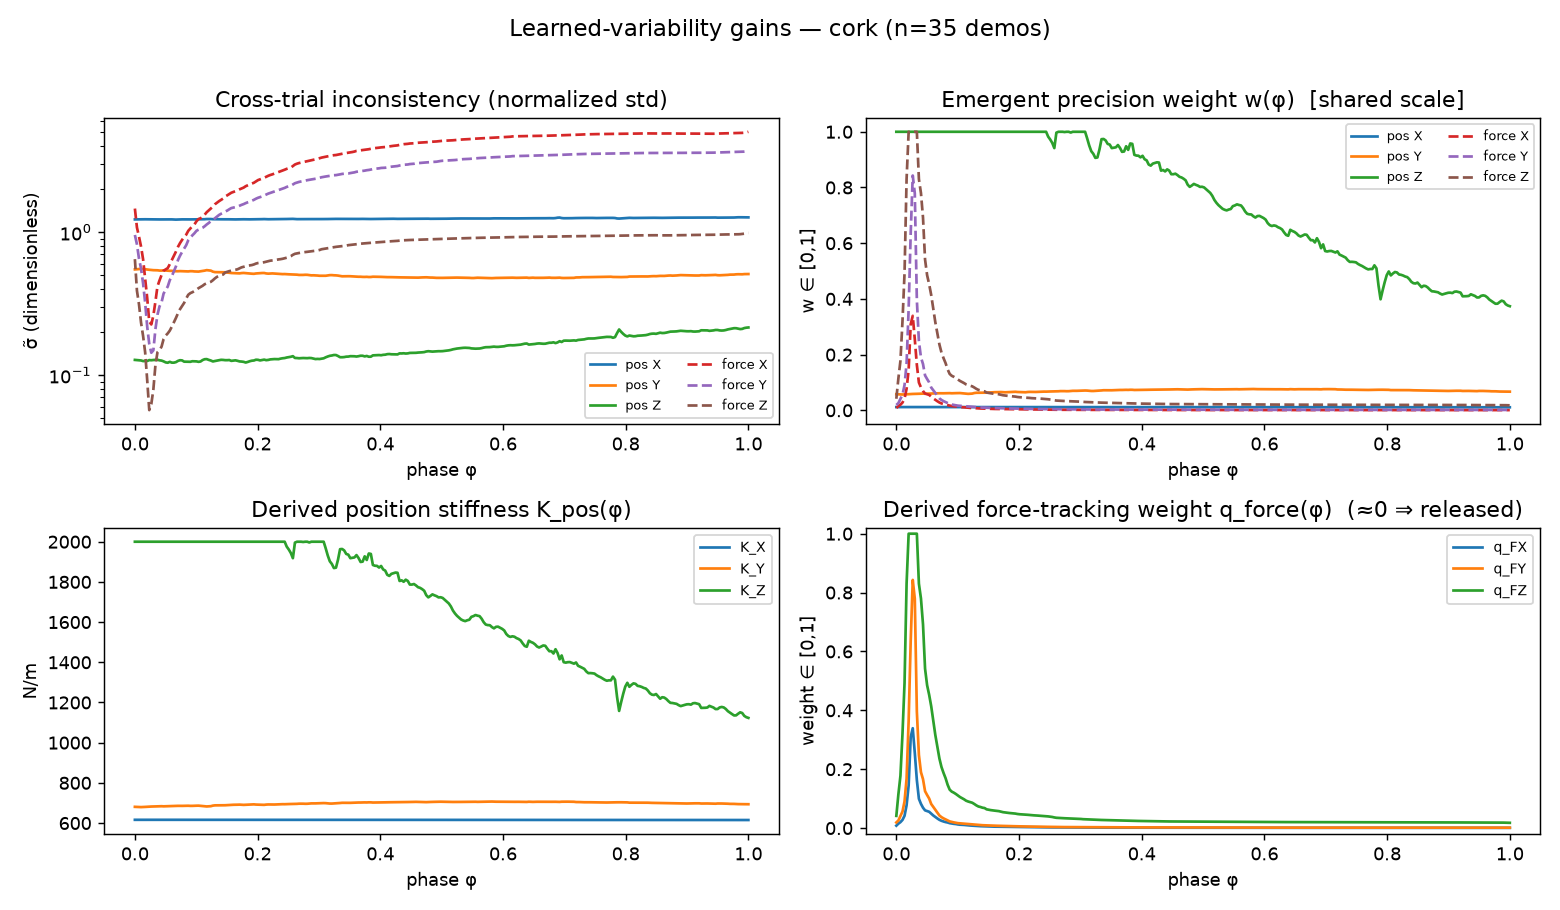
\includegraphics[width=0.95\textwidth]{variance_gains_cork.png}
\caption{Gains learned from the cork demonstrations. Top-left: cross-trial
inconsistency of each channel; top-right: the emergent precision weight $w(\phi)$;
bottom: the resulting position stiffness $K^{\text{pos}}(\phi)$ and the (near-zero)
force-tracking weight. The depth axis (blue) is regulated stiffly; force is
released. \emph{This split emerges from the data, not from tuning.}}
\label{fig:gains}
\end{figure}

The same procedure applied to the other two materials (Fig.~\ref{fig:gains_other})
yields the \emph{same qualitative structure} --- depth regulated, force released ---
but with \emph{material-specific magnitudes}, because the gains are computed from
each material's own demonstration. This is the gain-side counterpart of the
per-material force law of Section~\ref{sec:material}: one principle, three distinct
parameter sets.

\begin{figure}[h]
\centering
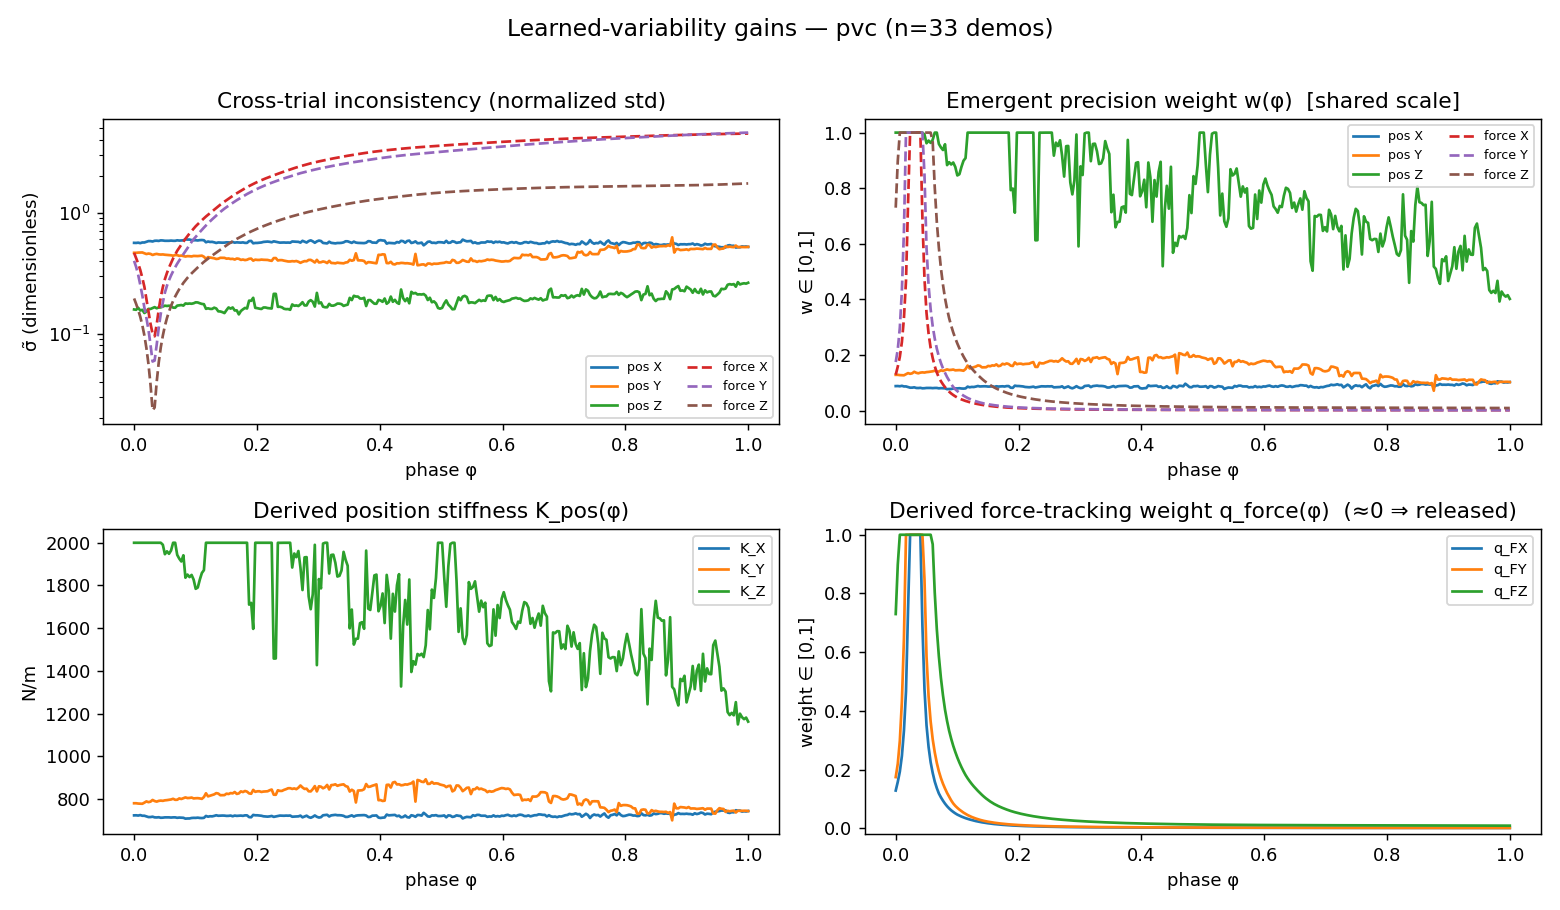
\includegraphics[width=0.83\textwidth]{variance_gains_pvc.png}\\[4pt]
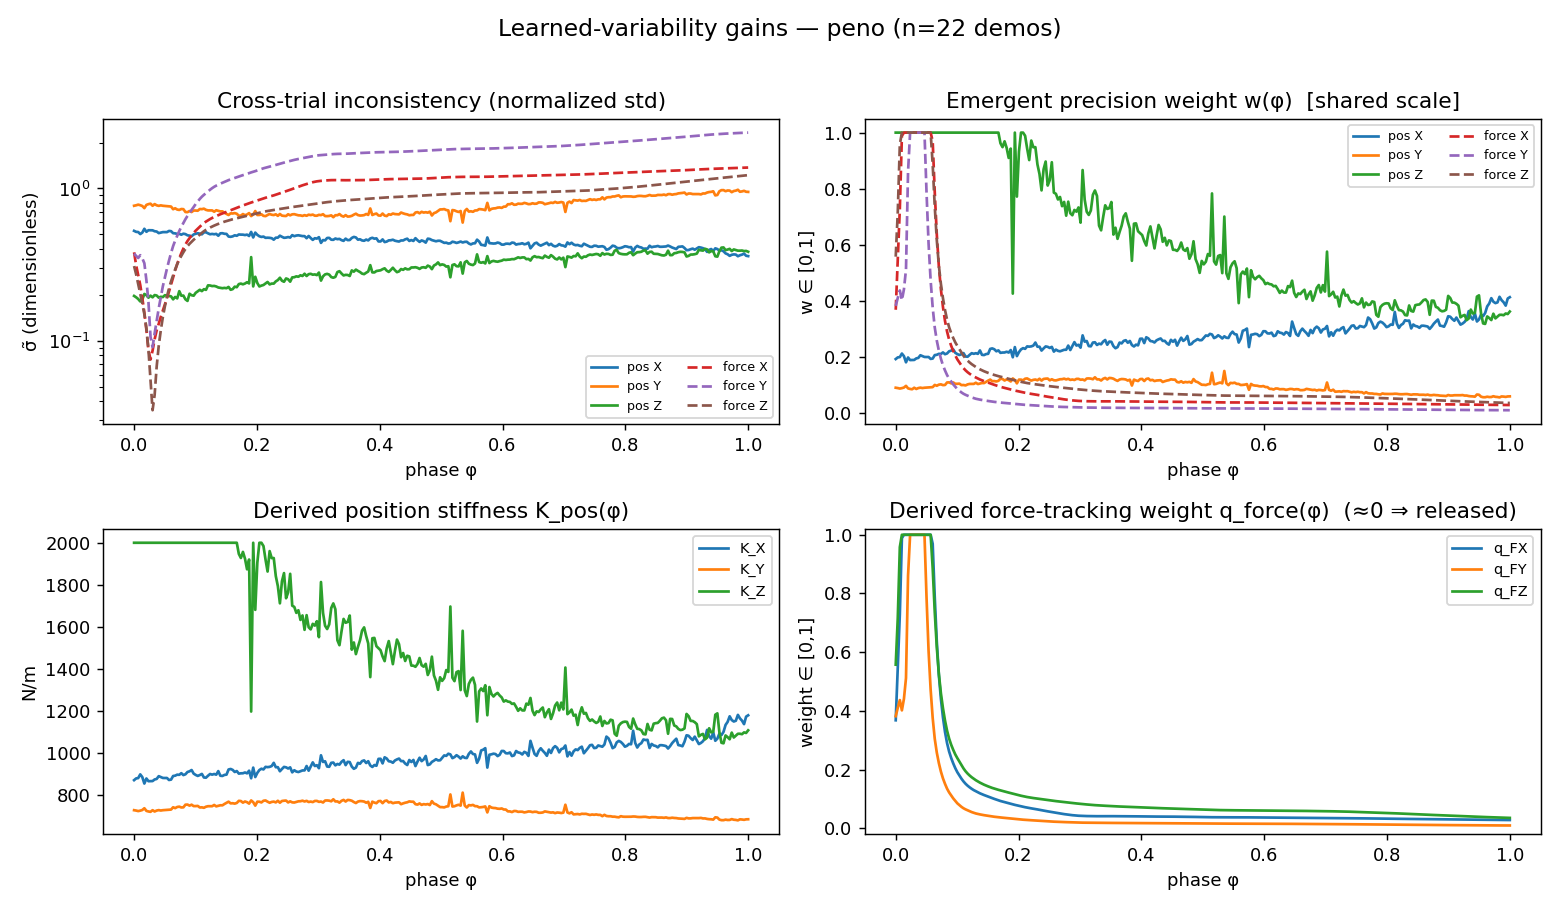
\includegraphics[width=0.83\textwidth]{variance_gains_peno.png}
\caption{Learned gains for PVC (top) and penoplex (bottom), produced by the same
precision rule \eqref{eq:precision} on each material's own demonstrations. The
structure is consistent with cork (Fig.~\ref{fig:gains}) --- the depth axis is
tracked stiffly and force is released --- while the stiffness magnitudes and
profiles differ per material, so the controller expresses material-specific
behaviour without any manual retuning.}
\label{fig:gains_other}
\end{figure}

\subsection{The online quadratic program (QP) for the gains}
\label{sec:qp}
At each control step, the gains are obtained from a small convex quadratic
program (QP) that \emph{blends} two objectives and respects two constraints:
\begin{equation}
\boxed{\;
\begin{aligned}
K^\star=\;\arg\min_{K\in\R^3}\;&
 q_f(\phi)\,\norm{K\odot\xt - F_d}_2^2
 \;+\;\big(1-q_f(\phi)\big)\,\norm{K - K^{\text{pos}}(\phi)}_2^2 \\
\text{s.t.}\;\;&
 K_{\min}\le K \le K_{\max},\qquad
 -F^{\text{bound}}_i \le K_i\,\xt_i \le F^{\text{bound}}_i\;\;\forall i .
\end{aligned}\;}
\label{eq:qp}
\end{equation}
Term by term:
\begin{itemize}[leftmargin=1.5em]
\item $\norm{K\odot\xt-F_d}_2^2$ is the \emph{force-consistency} cost ($\odot$ is
element-wise product): it pulls the impedance force $K\odot\xt\unit{N}$ to match the
desired force $F_d\unit{N}$. Its weight $q_f(\phi)\in[0,1]$ is the
\emph{force-precision} weight - small, because force is not reproducible
(Sec.~\ref{sec:analysis}).
\item $\norm{K-K^{\text{pos}}(\phi)}_2^2$ pulls the stiffness towards the
precision-derived value $K^{\text{pos}}\unit{N\,m^{-1}}$ of \eqref{eq:precision},
weighted by $1-q_f$. Because $q_f\!\to\!0$, this term dominates and the QP returns
$K\!\approx\!K^{\text{pos}}$: the controller tracks the precision-weighted
position skill.
\item The box constraint $K_{\min}\le K\le K_{\max}$ keeps stiffness in the
configured numerical range; hardware safety is not evaluated.
\item The constraint $|K_i\xt_i|\le F^{\text{bound}}_i$ bounds the
proportional residual-wrench component. The complete residual, including
integral and damping terms, is clipped separately. Neither bound directly
constrains measured contact force.
\end{itemize}
The damping follows from $K^\star$ by the fixed damping-ratio heuristic. The QP
has three decision variables and is evaluated at every simulated control step;
no wall-clock real-time guarantee is claimed. The raw solution is smoothed with
the preceding gain and then reprojected onto the current error-dependent
feasible interval before use.

\paragraph{Controlled comparison of learned variance structure.}
To test whether performance is associated with the selected precision
allocation, the identical task and controller are evaluated under four gain assignments:
(i) the identified precision; (ii) \emph{inverted} precision (regulating
directions that were inconsistent and relaxing those that were consistent);
(iii) precision \emph{permuted} across axes; and (iv) the original fixed-weight
QP with learned gains disabled. The saved artifact historically calls the
fourth condition ``direct force'', but it is not a measured-force feedback
controller. The metric is the \emph{cut-depth error} --- the
task-critical, demonstration-regulated axis --- evaluated over $12$ seeds with
randomised contact parameters (Fig.~\ref{fig:variance_comparison},
Table~\ref{tab:variance_comparison}).

Let $w(\phi)=[w_1(\phi),w_2(\phi),w_3(\phi)]^\top\in[0,1]^3$ be the
identified position-precision vector of \eqref{eq:precision}, and define the
affine normalisation of the Cartesian stiffness vector by
\begin{equation}
u(\phi)
=\frac{K^{\rm pos}(\phi)-K_{\min}\mathbf 1}
       {K_{\max}-K_{\min}}\in[0,1]^3,
\qquad
K^{\rm pos}(\phi)
=K_{\min}\mathbf1+(K_{\max}-K_{\min})u(\phi).
\label{eq:normalised_stiffness}
\end{equation}
Here $K^{\rm pos}=[K^{\rm pos}_1,K^{\rm pos}_2,K^{\rm pos}_3]^\top$ is the
Cartesian stiffness vector, $\mathbf 1\in\R^3$ is the all-ones vector, and the
scalar denominator is the full admissible stiffness range. Thus $u_i=0$ and
$u_i=1$ correspond respectively to $K_i^{\rm pos}=K_{\min}$ and
$K_i^{\rm pos}=K_{\max}$; $u$ is a dimensionless coordinate representation of
the commanded stiffness rather than an additional controller state.
Substitution of the learned gain law \eqref{eq:precision} into
\eqref{eq:normalised_stiffness} gives
\begin{equation}
\begin{aligned}
u_w(\phi)&=\eta_0\mathbf1+\eta_1w(\phi),\\
\eta_0&=\frac{K_{\rm floor}-K_{\min}}{K_{\max}-K_{\min}},\\
\eta_1&=\frac{K_{\max}-K_{\rm floor}}{K_{\max}-K_{\min}} .
\end{aligned}
\label{eq:identified_normalised_allocation}
\end{equation}
Accordingly, $u_w$ denotes the normalized Cartesian stiffness induced by the
precision weights obtained from the demonstrations.

The controlled comparison uses the exact transformations
\begin{equation}
\begin{aligned}
u^{\rm true}(\phi)&=u_w(\phi),\\
u^{\rm inv}(\phi)&=\mathbf 1-u_w(\phi),\\
u^{\rm perm}(\phi)&=\Pi(\phi)u_w(\phi),
\end{aligned}
\qquad
\Pi(\phi)^\top\Pi(\phi)=I ,
\label{eq:variance_assignments}
\end{equation}
The matched condition applies each learned component to its identified
Cartesian axis. The inverted condition acts componentwise and satisfies
\begin{equation}
u_i^{\rm inv}(\phi)=1-u_{w,i}(\phi),
\qquad
u_i^{\rm inv}-u_j^{\rm inv}
=-\big(u_{w,i}-u_{w,j}\big),
\label{eq:inverted_allocation_order}
\end{equation}
thereby reversing the component ordering about the midpoint of the admissible
normalized stiffness interval. The permuted condition preserves the
instantaneous multiset of components of $u_w$ but changes their Cartesian-axis
assignment. These transformations distinguish sensitivity to the learned
ordering from sensitivity to the learned axis association. The direct-force
condition is not an allocation transformation in this space: it disables the
learned-gain mode and applies the fixed force-QP weighting of the baseline
controller.

Write the identified allocation as
\begin{equation}
u_w(\phi)
=
\begin{bmatrix}
u_{w,x}(\phi)&u_{w,y}(\phi)&u_{w,z}(\phi)
\end{bmatrix}^{\top}.
\label{eq:allocation_axis_vector}
\end{equation}
For a bijection $\pi_\phi:\{1,2,3\}\rightarrow\{1,2,3\}$, define
\begin{equation}
[\Pi(\phi)]_{jk}
=
\begin{cases}
1,&k=\pi_\phi(j),\\
0,&\text{otherwise},
\end{cases}
\qquad j,k\in\{1,2,3\}.
\label{eq:permutation_definition}
\end{equation}
It follows that
\begin{equation}
[\Pi(\phi)u_w(\phi)]_j
=u_{w,\pi_\phi(j)}(\phi),
\qquad
\Pi(\phi)^\top\Pi(\phi)=I,
\qquad
\Pi(\phi)^{-1}=\Pi(\phi)^\top .
\label{eq:permutation_properties}
\end{equation}
Consequently, $\Pi(\phi)$ preserves the Euclidean norm and the multiset of
components of $u_w(\phi)$ while changing their Cartesian-axis assignment.
The dependence on $\phi$ permits the assignment to vary over task phase. In
the implemented shuffled condition, $\phi$ determines the pseudorandom seed
used to generate $\pi_\phi$. This comparison isolates the effect of the
learned axis assignment while preserving the instantaneous set of stiffness
allocations.

\begin{proposition}[Uniqueness of the matched allocation under the
precision-deviation functional]
\label{prop:precision_structure}
Consider the precision-allocation functional
\begin{equation}
\mathcal J[u]
=\frac12\int_0^1
\big(u(\phi)-u_w(\phi)\big)^\top
H(\phi)
\big(u(\phi)-u_w(\phi)\big)\,d\phi ,
\qquad H(\phi)=H(\phi)^\top\succ0 .
\label{eq:precision_functional}
\end{equation}
Among all measurable allocations $u:[0,1]\rightarrow[0,1]^3$, the matched
assignment $u^{\rm true}=u_w$ is the unique minimiser of
\eqref{eq:precision_functional}, up to sets of zero measure.
The excess costs of the inverted and permuted structures are
\begin{align}
\mathcal G_{\rm inv}
&=\frac12\int_0^1
(\mathbf1-2u_w)^\top H(\mathbf1-2u_w)\,d\phi ,
\label{eq:inverted_excess}\\
\mathcal G_{\rm perm}
&=\frac12\int_0^1
(\Pi u_w-u_w)^\top H(\Pi u_w-u_w)\,d\phi .
\label{eq:permuted_excess}
\end{align}
Both are strictly positive whenever the transformation changes a
task-weighted component of $u_w$ on a phase interval of non-zero measure.
\end{proposition}
\begin{proof}
Since $H(\phi)\succ0$, its smallest eigenvalue
$h_{\min}(\phi)=\lambda_{\min}(H(\phi))$ is positive and
\begin{equation}
\mathcal J[u]
\ge\frac12\int_0^1
h_{\min}(\phi)\norm{u(\phi)-u_w(\phi)}_2^2\,d\phi
\ge0 .
\label{eq:precision_lower_bound}
\end{equation}
The lower bound is attained by $u=u_w$, for which
$\mathcal J[u_w]=0$. Equality for another allocation requires
$u(\phi)=u_w(\phi)$ almost everywhere, which proves uniqueness. Substitution of
$u^{\rm inv}=\mathbf1-u_w$ and $u^{\rm perm}=\Pi u_w$ into
\eqref{eq:precision_functional} gives
\eqref{eq:inverted_excess} and \eqref{eq:permuted_excess}. Positive
definiteness of $H$ makes either integral strictly positive when its difference
vector is non-zero on a set of non-zero measure.
\end{proof}

Define the allocation error
\begin{equation}
e_u(\phi)=u(\phi)-u_w(\phi)
=
\begin{bmatrix}
e_x(\phi)&e_y(\phi)&e_z(\phi)
\end{bmatrix}^{\top}.
\label{eq:allocation_error}
\end{equation}
Then the integrand of \eqref{eq:precision_functional} is the quadratic form
\begin{equation}
\frac12 e_u^\top H e_u
=\frac12\sum_{j=1}^{3}\sum_{k=1}^{3}
H_{jk}(\phi)e_j(\phi)e_k(\phi).
\label{eq:H_quadratic_expansion}
\end{equation}
Here $H:[0,1]\rightarrow\mathbb S_{++}^{3}$ is a measurable,
phase-dependent task-relevance metric on the allocation space. Its diagonal
entries weight axis-specific allocation errors, whereas its off-diagonal
entries encode cross-axis coupling. The condition $H(\phi)\succ0$ means
\begin{equation}
v^\top H(\phi)v>0
\quad\text{for every non-zero }v\in\R^3,
\label{eq:H_positive_definite}
\end{equation}
and is the condition required for the uniqueness result in
Proposition~\ref{prop:precision_structure}. For the cutting task, greater
depth-axis relevance may be represented through the corresponding entries of
$H(\phi)$.

The matrix $H(\phi)$ is an assumed metric defining the quadratic allocation
functional; it is not estimated from the demonstrations, numerically specified
in the experiments, or evaluated by the controller. Consequently,
Proposition~\ref{prop:precision_structure} establishes only that $u_w$
uniquely minimizes the defined weighted deviation from $u_w$. It does not
establish optimality with respect to cutting error, interaction force, or a
general closed-loop performance functional. The physical consequence of the
matched allocation is instead evaluated by the paired closed-loop experiment
below.

For controller condition $c$ and randomised-physics seed $s$, the reported
cut-depth metric is
\begin{equation}
E_{s,c}^{z}
=10^3\sqrt{\frac{1}{t_{f,s}}
\int_0^{t_{f,s}}
\big(x_{d,z}^{(s,c)}(t)-x_z^{(s,c)}(t)\big)^2\,dt}
\quad[\mathrm{mm}],
\label{eq:depth_rmse}
\end{equation}
where $t_{f,s}$ is the episode duration, $x_{d,z}$ is desired scalpel depth, $x_z$
is measured depth, and the factor $10^3$ converts metres to millimetres. The
same randomised mass, friction, contact parameters and initial perturbation are
used for all conditions within seed $s$, so the paired difference
\begin{equation}
G_{s,c}=E_{s,c}^{z}-E_{s,{\rm true}}^{z}
\label{eq:paired_difference}
\end{equation}
removes seed-specific physics shared by the two runs. Positive
$G_{s,c}$ means that condition $c$ has larger cut-depth error than the
identified precision assignment.

\begin{figure}[h]
\centering
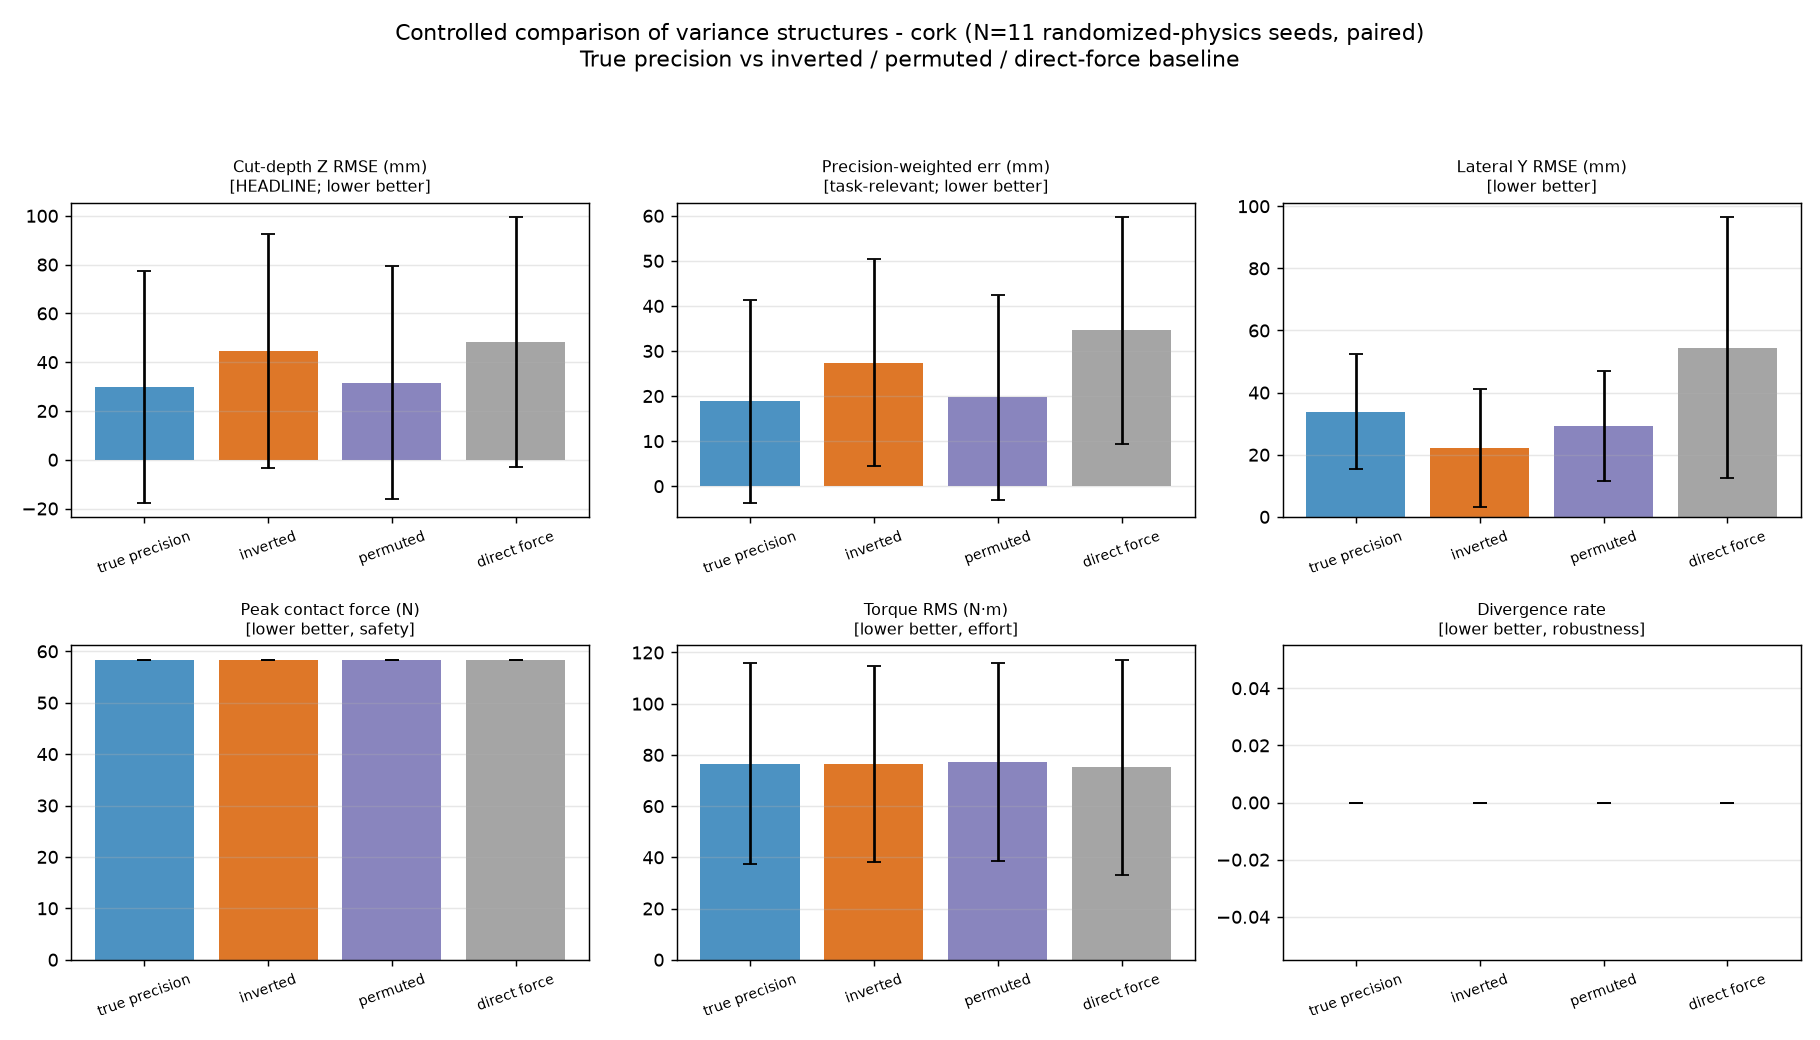
\includegraphics[width=0.97\textwidth]{study_variance_comparison_cork.png}
\caption{Controlled comparison of gain assignments on cork ($N_{\rm seed}=12$
randomised-physics seeds,
paired). Only the identified precision attains low cut-depth error; inverting or
permuting the learned structure degrades it. Bars denote mean$\pm$std.}
\label{fig:variance_comparison}
\end{figure}

\begin{table}[h]
\centering
\begin{tabular}{lccc}
\toprule
Gain assignment & depth RMSE (mm) & identified reduction & Wilcoxon $p$ \\
\midrule
\textbf{Identified precision} & $\mathbf{10.9 \pm 2.5}$ & --- & --- \\
Permuted precision & $14.7 \pm 2.9$ & $+26\%$ & $0.001$ \\
Inverted precision & $20.7 \pm 4.0$ & $+47\%$ & $0.001$ \\
Direct force-tracking & $20.9 \pm 5.9$ & $+48\%$ & $0.001$ \\
\bottomrule
\end{tabular}
\caption{The identified precision attains the lowest cut-depth error on all $11$
stable seeds and reduces error by $26$--$48\%$ relative to the three comparator
assignments ($p=0.001$, the smallest value attainable by the paired Wilcoxon
test at this sample size). This isolates the identified \emph{variance structure},
rather than gain adaptation in general, as the determinant of task performance.}
\label{tab:variance_comparison}
\end{table}

For the $n_{\rm pair}=11$ seeds that were stable in every paired condition, the table
reports
\begin{equation}
\bar E_c=\frac1{n_{\rm pair}}\sum_{s=1}^{n_{\rm pair}}E_{s,c}^{z},
\qquad
s_c=\sqrt{\frac{1}{n_{\rm pair}-1}\sum_{s=1}^{n_{\rm pair}}
\big(E_{s,c}^{z}-\bar E_c\big)^2},
\label{eq:sample_statistics}
\end{equation}
where $\bar E_c$ and $s_c$ are respectively the sample mean and sample standard
deviation for condition $c$. The percentage shown in the third column is the
error reduction achieved by the identified assignment relative to comparator
$c$,
\begin{equation}
R_c=100\,
\frac{\bar E_c-\bar E_{\rm true}}{\bar E_c}\quad[\%],
\label{eq:relative_reduction}
\end{equation}
which gives $26\%$, $47\%$ and $48\%$ for the permuted, inverted and
direct-force conditions. This denominator explains why these percentages are
reductions relative to each comparator rather than percentage increases
relative to the identified mean.

\begin{proposition}[Paired dominance in the evaluated seeds]
\label{prop:paired_variance}
For each of the three comparator conditions, the evaluated stable pairs satisfy
$G_{s,c}>0$ for all $s\in\{1,\ldots,11\}$. The exact two-sided paired
Wilcoxon signed-rank test therefore gives
\begin{equation}
p_{\rm exact}=2^{1-n_{\rm pair}}
=2^{-10}=0.0009765625\approx0.001 .
\label{eq:wilcoxon_exact}
\end{equation}
\end{proposition}
\begin{proof}
Let $\varrho_s$ be the rank of $|G_{s,c}|$ among the
$n_{\rm pair}$ non-zero paired
differences and define the negative signed-rank statistic
\begin{equation}
W^-_c=\sum_{s=1}^{n_{\rm pair}}\varrho_s\,
\mathbb 1_{\{G_{s,c}<0\}} .
\label{eq:wilcoxon_statistic}
\end{equation}
Because every observed difference is positive, $W^-_c=0$. Under the Wilcoxon
null hypothesis of a distribution symmetric about zero, each of the
$2^{n_{\rm pair}}$ sign
assignments is equally likely. Only the all-positive and all-negative
assignments are at least as extreme as the observed one, so the two-sided exact
probability is
$2/2^{n_{\rm pair}}=2^{1-n_{\rm pair}}$. Substitution of
$n_{\rm pair}=11$ yields
\eqref{eq:wilcoxon_exact}.
\end{proof}

Proposition~\ref{prop:paired_variance} is an exact statement about the evaluated
paired seeds and rejects the zero-median-difference null at the reported sample
size. Together with Proposition~\ref{prop:precision_structure}, it links the
analytical consequence of matching the learned precision allocation to the
observed closed-loop reduction in the task-critical error, without treating the
finite simulation sample as a universal proof for all contact conditions.

% ============================================================================
\section{State-driven task parametrization}
% ============================================================================
\label{sec:phase}
\subsection{Theoretical motivation}
Contact-rich skill execution involves two distinct objects: the geometric and
interaction structure of the skill, and the rate at which that structure is
traversed.  A purely temporal reference conflates them by imposing
$x_d(t)=x_r(t/T_d)$.  Under free motion this may be adequate; under contact,
however, the realised state is affected by material deformation, friction,
actuator limits, external perturbations and passivity intervention.  The
temporal phase can therefore continue to advance while the physical system
remains near an earlier task state.

Let
\begin{equation}
z(t)=\begin{bmatrix}x(t)^\top&\norm{F(t)}_2\end{bmatrix}^{\!\top},
\qquad
z_r(\phi)=
\begin{bmatrix}x_r(\phi)^\top&\norm{F_r(\phi)}_2\end{bmatrix}^{\!\top}
\label{eq:phase_augmented_state}
\end{equation}
denote the measured and reference task states, respectively.  The phase
consistent with the realised task state is the local projection
\begin{equation}
\phi^\star(t)\in
\arg\min_{\varphi\in\mathcal I(t)}
\norm{W\big(z_r(\varphi)-z(t)\big)} ,
\label{eq:ideal_state_phase}
\end{equation}
where $W$ is a dimensional normalisation/weighting matrix and
$\mathcal I(t)\subseteq[0,1]$ restricts the admissible branch of the reference
curve.  For a clock phase $\phi_c(t)=t/T_d$, define the synchronisation error
$e_\phi(t)=\phi_c(t)-\phi^\star(t)$.  If $x_r$ is differentiable, the reference
displacement induced solely by this loss of synchronisation satisfies the
first-order relation
\begin{equation}
x_r(\phi_c)-x_r(\phi^\star)
=x'_r(\phi^\star)e_\phi+\mathcal O(e_\phi^2).
\label{eq:phase_desynchronisation}
\end{equation}
Thus a phase error is converted directly into a Cartesian reference error,
scaled by the local path tangent.  During contact, this error is further mapped
through the impedance into a commanded wrench.  Continuing a clock-driven
reference during arrested motion can consequently increase both tracking
error and demanded interaction power, even when the geometric prior itself is
appropriate.

State-driven parametrisation addresses this synchronisation problem by treating
phase as an internal progress coordinate inferred from the realised task
state, rather than as elapsed time alone.  This has three theoretical
consequences.  First, it separates the phase-indexed task manifold
$\mathcal M=\{z_r(\phi):\phi\in[0,1]\}$ from its temporal traversal law.
Second, local projection onto $\mathcal M$ makes reference selection dependent
on physical task progress.  Third, constraining the phase law to be
non-negative preserves the causal ordering of approach, engagement, cutting
and termination.  For the present controller, state projection, nominal
temporal progression and the energy-tank gate are combined in a sampled-data
phase law; the precise construction follows.

\subsection{Phase-domain skill representation}
Let the learned behaviour prior be the phase-indexed curve
\begin{equation}
\mathcal B(\phi)
=\big(x_r(\phi),\,x'_r(\phi),\,F_r(\phi),\,K(\phi),\,D(\phi)\big),
\qquad \phi\in[0,1],
\label{eq:phase_prior}
\end{equation}
where a prime denotes differentiation with respect to phase.  For any absolutely continuous,
non-decreasing phase $\phi(t)$, the commanded position and its physically
consistent velocity satisfy
\begin{equation}
x_d(t)=x_r(\phi(t)),\qquad
\dot x_d(t)=x'_r(\phi(t))\dot\phi(t).
\label{eq:phase_chain_rule}
\end{equation}
Temporal scaling changes $\dot x_d$ without changing the image of the path.
If the demonstration has
duration $T_d$ and the requested dimensionless speed multiplier is
$s_\phi>0$, the ungated nominal phase rate is
\begin{equation}
\dot\phi_{\rm nom}=\frac{s_\phi}{T_d},
\qquad
T_{\rm exec}^{\rm nom}=\frac{T_d}{s_\phi}.
\label{eq:nominal_phase_rate}
\end{equation}
This defines the nominal traversal law prior to state and passivity adaptation.

\subsection{State-to-phase observation}
At controller sample $k$, let $\phi_k$ be the phase used to evaluate the prior,
$x_k$ the measured TCP position, and $F_k$ the filtered measured interaction
force.  The stored reference contains $N$ uniformly spaced knots
\begin{equation}
\Phi_N=\left\{\phi^{(j)}=\frac{j}{N-1}:j=0,\ldots,N-1\right\}.
\end{equation}
Rather than searching the entire curve, the implementation forms the local
candidate set
\begin{equation}
\mathcal C_k
=\left\{\phi^{(j)}\in\Phi_N:
\max(0,\phi_k-\ell_\phi^-)\leq\phi^{(j)}
\leq\min(1,\phi_k+\ell_\phi^+)\right\},
\label{eq:phase_candidates}
\end{equation}
where $\ell_\phi^-=\ell_\phi^+=0.1$.  The backward branch permits measured
lag to retard the reference; monotonicity is imposed by the phase dynamics
rather than by excluding earlier candidates.
The normalising scales used in the implementation are
\begin{equation}
\rho_x=\norm{x_r(1)-x_r(0)}_2+\varepsilon_x,\qquad
\rho_F=\max_{\phi^{(j)}\in\Phi_N}\norm{F_r(\phi^{(j)})}_2+\varepsilon_F,
\label{eq:phase_scales}
\end{equation}
with $\varepsilon_x,\varepsilon_F>0$.  Define the contact indicator
\begin{equation}
c_k=\mathbb 1_{\{\norm{F_k}_2>F_{\rm contact}\}}.
\label{eq:contact_indicator}
\end{equation}
The phase-observation cost is
\begin{equation}
J_k(\varphi)=
\begin{cases}
\displaystyle
\frac{\norm{x_r(\varphi)-x_k}_2}{\rho_x},
&c_k=0,\\[2mm]
\displaystyle
\frac{1}{2}\frac{\norm{x_r(\varphi)-x_k}_2}{\rho_x}
+\frac{1}{2}
\frac{\left|\norm{F_r(\varphi)}_2-\norm{F_k}_2\right|}{\rho_F},
&c_k=1.
\end{cases}
\label{eq:phase_observation_cost}
\end{equation}
The observed progress is the discrete nearest point
\begin{equation}
\hat\phi_k\in\arg\min_{\varphi\in\mathcal C_k}J_k(\varphi),
\label{eq:phase_estimator}
\end{equation}
with the first minimising knot resolving ties.  Retaining the position term
during contact mitigates non-uniqueness of the force-magnitude map
$\phi\mapsto\norm{F_r(\phi)}_2$.  The bounded search interval selects a local
branch when the reference curve is not globally injective.

\subsection{Sampled-data phase dynamics}
Let $h_c$ denote the controller period and let the energy-tank gate
$\gamma_{T,k}\in[0,1]$ be defined by \eqref{eq:tank_disc}.  The nominal
increment available at sample $k$ is
\begin{equation}
\Delta\phi_k^{\rm nom}
=h_c\gamma_{T,k}\dot\phi_{\rm nom}
=\gamma_{T,k}\frac{s_\phi h_c}{T_d}.
\label{eq:nominal_phase_increment}
\end{equation}
The raw state correction and its implemented increment limiter are
\begin{align}
r_k&=h_c k_\phi(\hat\phi_k-\phi_k),
\qquad k_\phi=2.0\unit{s^{-1}},\\
\delta\phi_k
&=\operatorname{sat}_{[-\Delta\phi_k^{\rm nom},
\,2\Delta\phi_k^{\rm nom}]}(r_k),
\label{eq:phase_correction}
\end{align}
where
$\operatorname{sat}_{[a,b]}(z)=\min\{b,\max\{a,z\}\}$.
The complete recursion is therefore
\begin{equation}
\boxed{\quad
\phi_{k+1}
=\Pi_{[0,1]}\!\left(
\phi_k+\Delta\phi_k^{\rm nom}+\delta\phi_k
\right),\quad}
\label{eq:phase}
\end{equation}
where $\Pi_{[0,1]}(z)=\min\{1,\max\{0,z\}\}$.  All terms in the recursion are
dimensionless phase increments.

\begin{proposition}[Monotonicity and bounded phase rate]
\label{prop:phase_monotonicity}
For $\phi_0\in[0,1]$, $\gamma_{T,k}\in[0,1]$, and
$\dot\phi_{\rm nom}\geq0$, recursion \eqref{eq:phase} satisfies
\begin{equation}
0\leq\phi_k\leq1,\qquad
0\leq\phi_{k+1}-\phi_k
\leq3h_c\gamma_{T,k}\dot\phi_{\rm nom}.
\label{eq:phase_increment_bound}
\end{equation}
\end{proposition}
\begin{proof}
Projection gives $0\leq\phi_{k+1}\leq1$.  From
\eqref{eq:phase_correction},
$-\Delta\phi_k^{\rm nom}\leq\delta\phi_k
\leq2\Delta\phi_k^{\rm nom}$, hence the unprojected increment belongs to
$[0,3\Delta\phi_k^{\rm nom}]$.  Projection at the upper endpoint can only
reduce a non-negative increment, proving \eqref{eq:phase_increment_bound}.
\end{proof}

Setting $k_\phi=0$ removes state matching and gives a tank-gated clock.
Setting additionally $\gamma_{T,k}=1$ gives uniform time parametrisation.
For $k_\phi>0$, the bidirectional state observation retards phase when
$\hat\phi_k<\phi_k$ and accelerates it when $\hat\phi_k>\phi_k$.  The lower
saturation limit permits complete cancellation of the nominal increment but
precludes reversal; the upper limit bounds the total rate by three times the
tank-gated nominal rate.  In addition, as $T_k\downarrow T_{\min}$,
$\gamma_{T,k}\downarrow0$, which drives both
$\Delta\phi_k^{\rm nom}$ and its permitted correction to zero.  This
separation prevents phase reversal while coupling task timing to the available
energy budget.  The implemented construction is therefore a
\emph{bidirectionally corrected, tank-gated state-dependent parametrisation}.  It
provides temporal scaling through $s_\phi$, measured-state correction through
\eqref{eq:phase_estimator}, monotone bounded progression through
\eqref{eq:phase}, and energy-dependent slowing through $\gamma_{T,k}$.

\subsection{Controlled phase--state desynchronisation}
\label{sec:holdback}
Workpiece motion changes contact geometry but does not necessarily create a
repeatable lag along the cutting path.  A separate exogenous perturbation was
therefore introduced to test the causal property for which state-driven
parametrisation was designed.  Let
\begin{equation}
\hat t_r(\phi)=
\frac{x'_r(\phi)}{\norm{x'_r(\phi)}_2+\varepsilon_t}
\label{eq:path_tangent_unit}
\end{equation}
denote the regularised unit tangent to the reference path.  During the
prescribed interval $[t_a,t_b]$, the MuJoCo external-force input on the scalpel
body is augmented by
\begin{equation}
f_h(t,\phi)=
-F_h\,\hat t_r(\phi)\,
\mathbb 1_{\{t_a\leq t\leq t_b\}},
\qquad
F_h=120\unit{N},\quad
(t_a,t_b)=(0.9,1.4)\unit{s}.
\label{eq:holdback_force}
\end{equation}
This \emph{holdback force} acts opposite to instantaneous path progression and
is added to, rather than substituted for, the identified material reaction.
It enters the robot dynamics through the physical external-wrench channel; it
does not modify $\phi$, $\hat\phi$ or $\dot\phi$ numerically.  Its causal route
is therefore
\[
f_h\longrightarrow(x,\dot x,F)
\longrightarrow\hat\phi
\longrightarrow\dot\phi .
\]
The perturbation is not part of nominal cutting or of the learned controller.
It is a validation input analogous to an impulse or step disturbance in a
closed-loop robustness experiment.  Runtime configuration consequently
defaults it to disabled; its enable flag, amplitude and time interval are
independent of the switch selecting state-driven or time-driven phase.

\subsection{Factorial runtime ablation}
The evaluation crossed three binary factors: static versus vertically moving
workpiece, nominal versus holdback-perturbed execution, and state-driven versus
time-driven phase.  The time-driven condition sets the state-correction term to
zero while retaining the learned variable impedance, material model,
energy-tank gate and torque projection.  Thus the comparison does not remove a
safety mechanism.  Five paired randomised-physics seeds were used; within each
scenario and seed the two phase laws received identical friction, contact
solver parameters, material mass and initial joint perturbation.

The static and moving conditions use the same world-frame desired position and
velocity trajectories. Workpiece motion is applied only to the simulated
material joint and is not added to either reference; it is therefore an
external geometric perturbation, matching the experimental convention used
for the holdback force. The material surface used by the contact model remains
live, so only the environment geometry changes.

\begin{table}[h]
\centering
\small
\caption{Factorial task-parametrisation comparison. Entries are mean
$\pm$ standard deviation over $N=5$ paired seeds; S and T denote state-driven
and time-driven phase, respectively.}
\label{tab:phase_factorial}
\begin{tabular}{lccccc}
\toprule
Workpiece & Holdback &
\multicolumn{2}{c}{Cut-depth RMSE [mm]} &
\multicolumn{2}{c}{Position RMSE [mm]} \\
& & S & T & S & T \\
\midrule
Static & off & $2.533\pm1.031$ & $2.598\pm1.140$
             & $17.944\pm18.861$ & $20.917\pm24.734$ \\
Static & on  & $2.957\pm0.888$ & $3.171\pm1.407$
             & $76.555\pm30.224$ & $82.926\pm46.662$ \\
Moving & off & $8.816\pm8.069$ & $8.816\pm8.286$
             & $32.298\pm32.363$ & $28.364\pm32.250$ \\
Moving & on  & $9.272\pm7.689$ & $9.501\pm7.853$
             & $75.904\pm18.168$ & $63.490\pm31.489$ \\
\bottomrule
\end{tabular}
\end{table}

\begin{figure}[h]
\centering
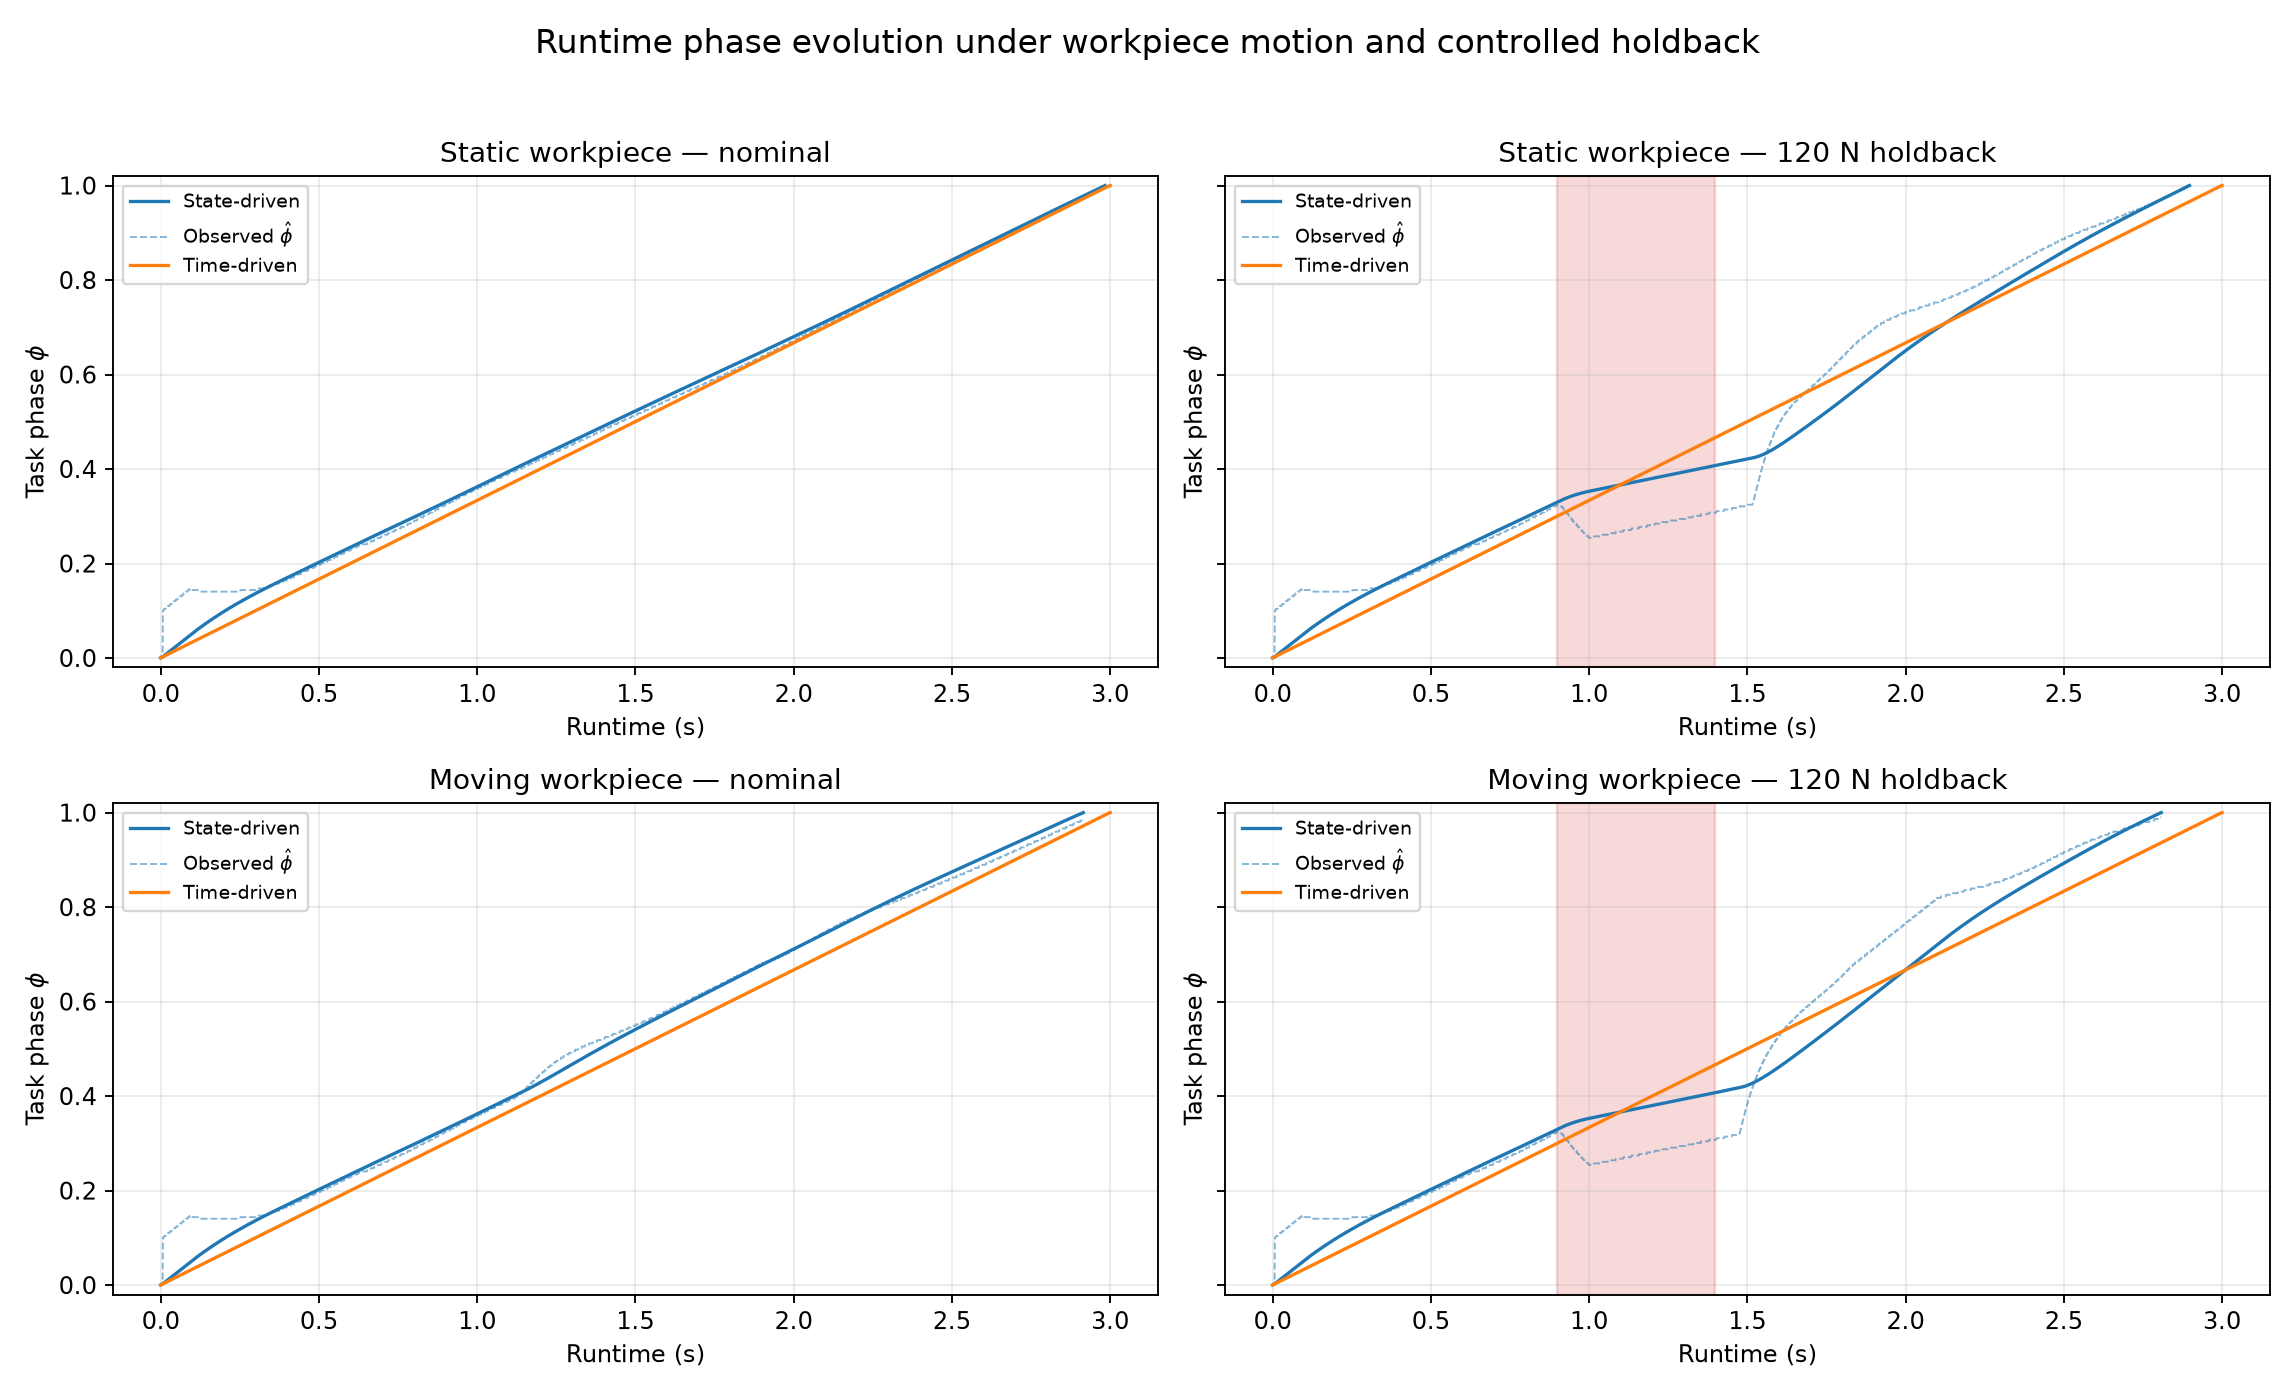
\includegraphics[width=\textwidth]{task_parametrization_runtime_cork.png}
\caption{Representative runtime phase evolution for static and moving
workpieces, with and without the controlled holdback.  The red interval is the
physical perturbation \eqref{eq:holdback_force}.  In nominal runs the two laws
remain close.  Under holdback, the measured projection $\hat\phi$ falls behind
the commanded phase and the state-driven law retards progress, whereas the
time-driven phase continues at its clock rate.}
\label{fig:phase_runtime_factorial}
\end{figure}

\begin{figure}[h]
\centering
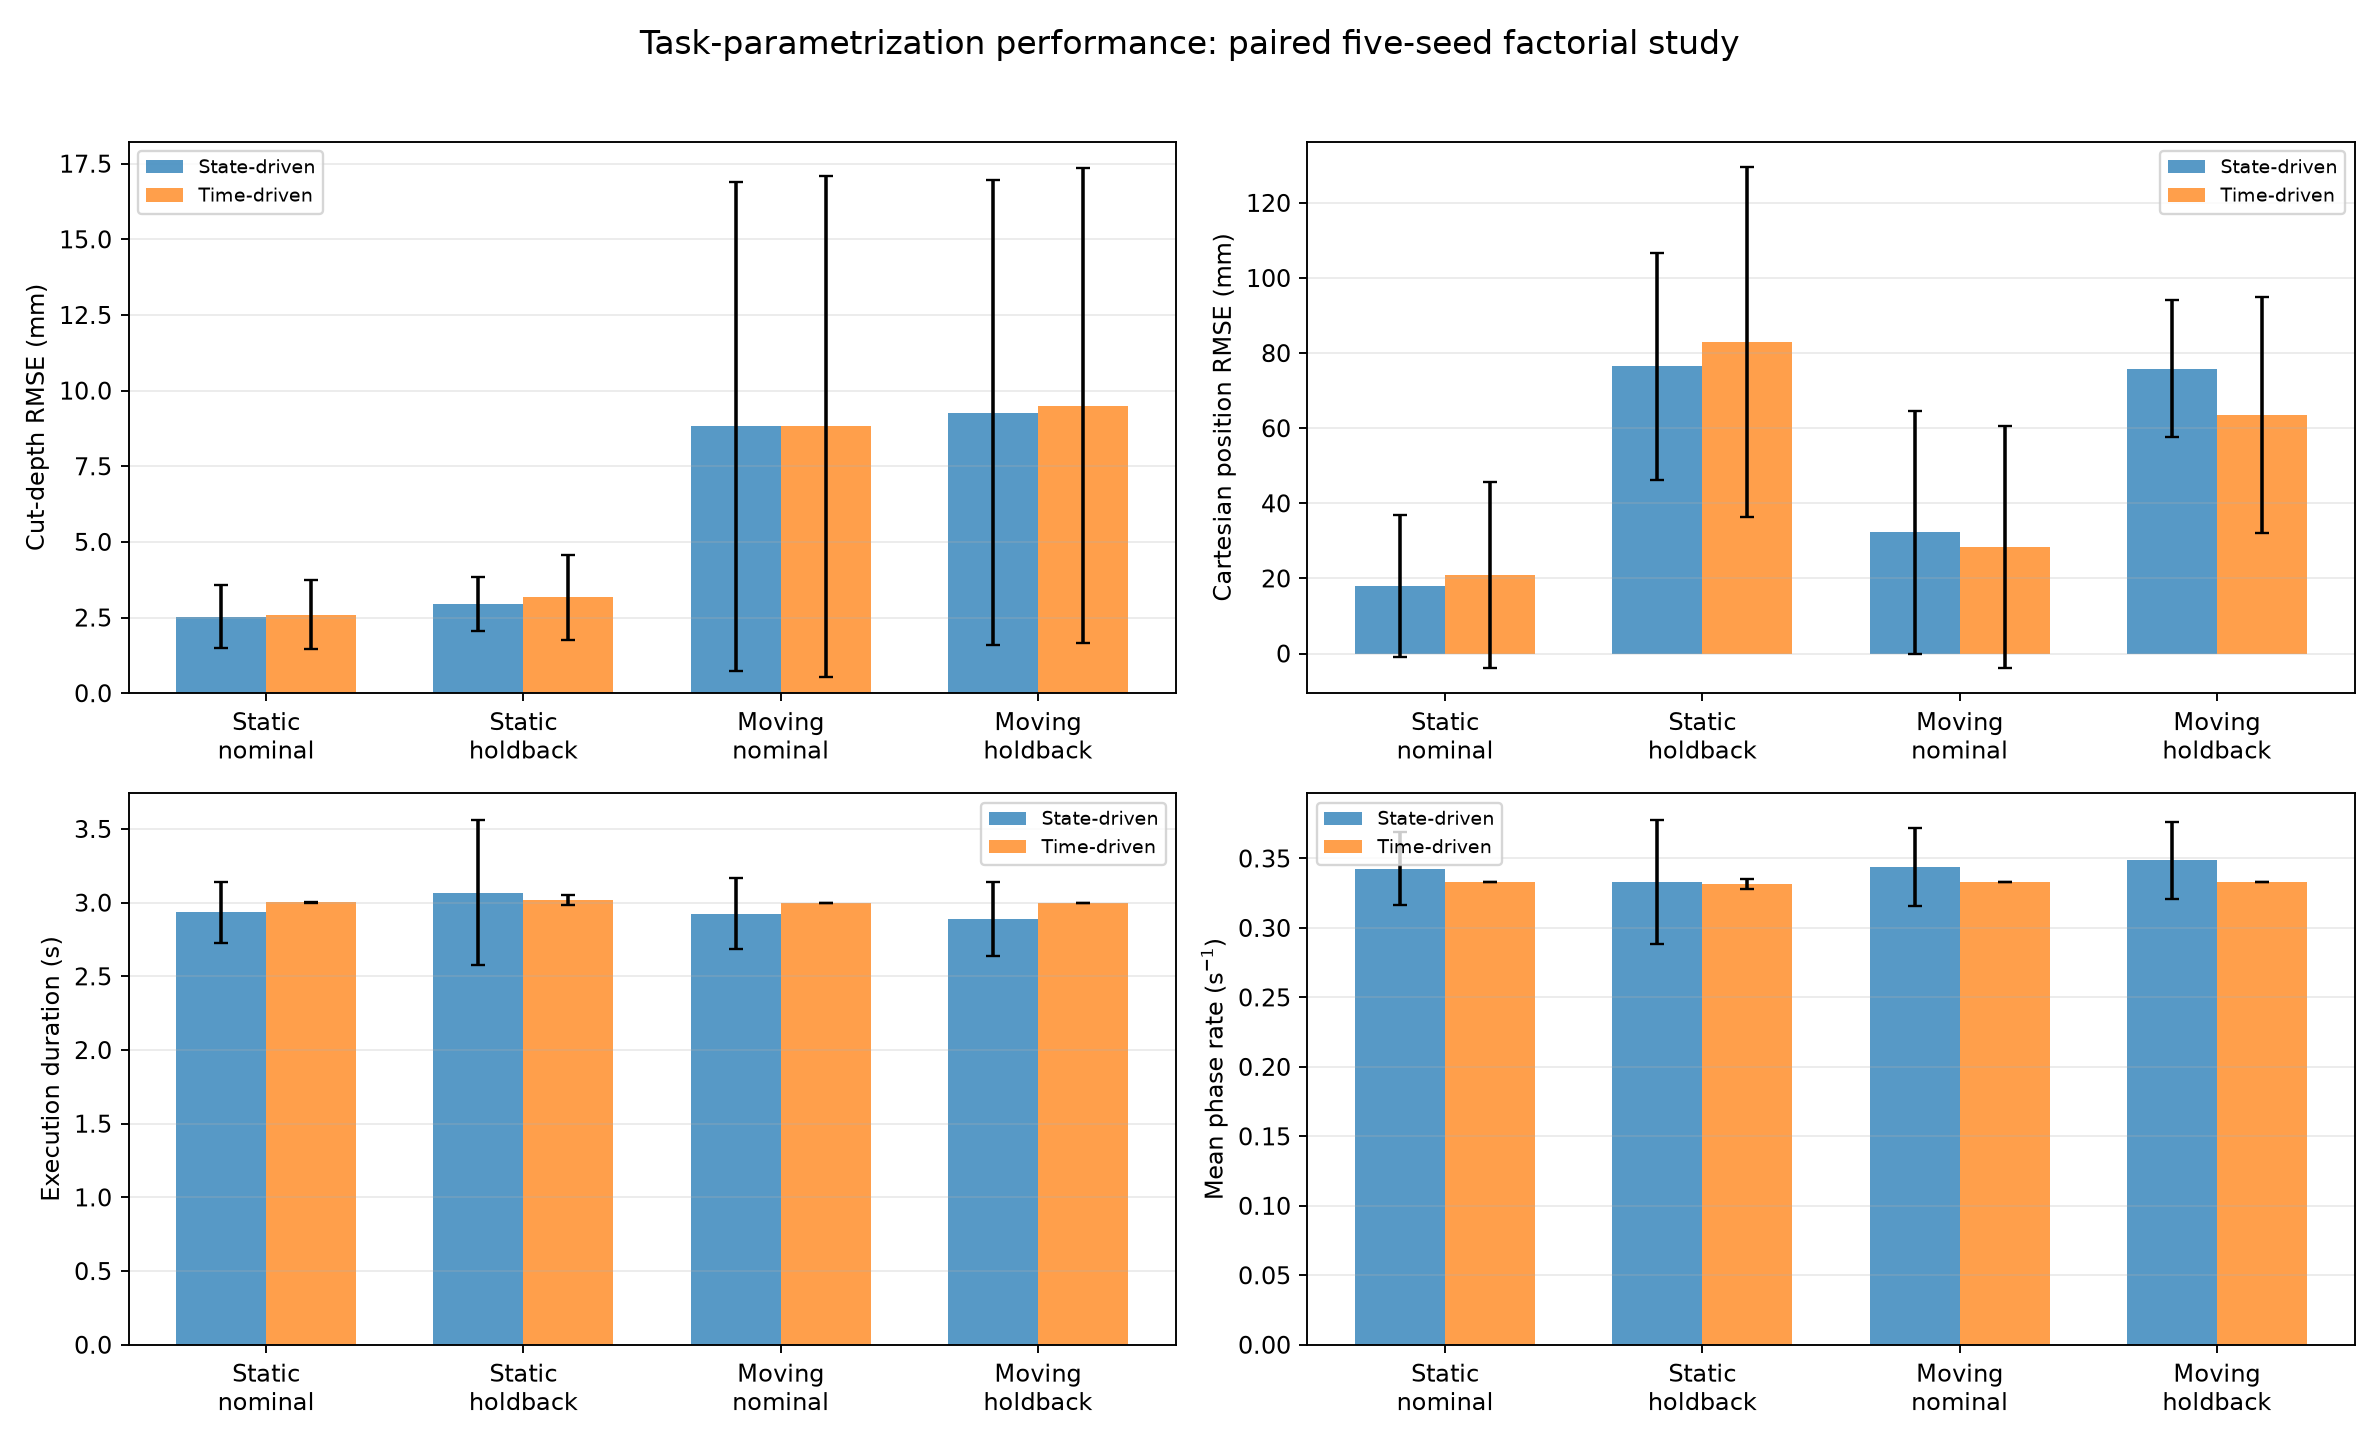
\includegraphics[width=\textwidth]{task_parametrization_performance_cork.png}
\caption{Performance over the complete factorial study. Error bars show one
standard deviation across paired randomised-physics seeds.  State-dependent
timing trades execution time for synchronisation when measured progress lags;
its rate can also exceed the clock rate when the state projection is ahead.}
\label{fig:phase_performance_factorial}
\end{figure}

\begin{figure}[h]
\centering
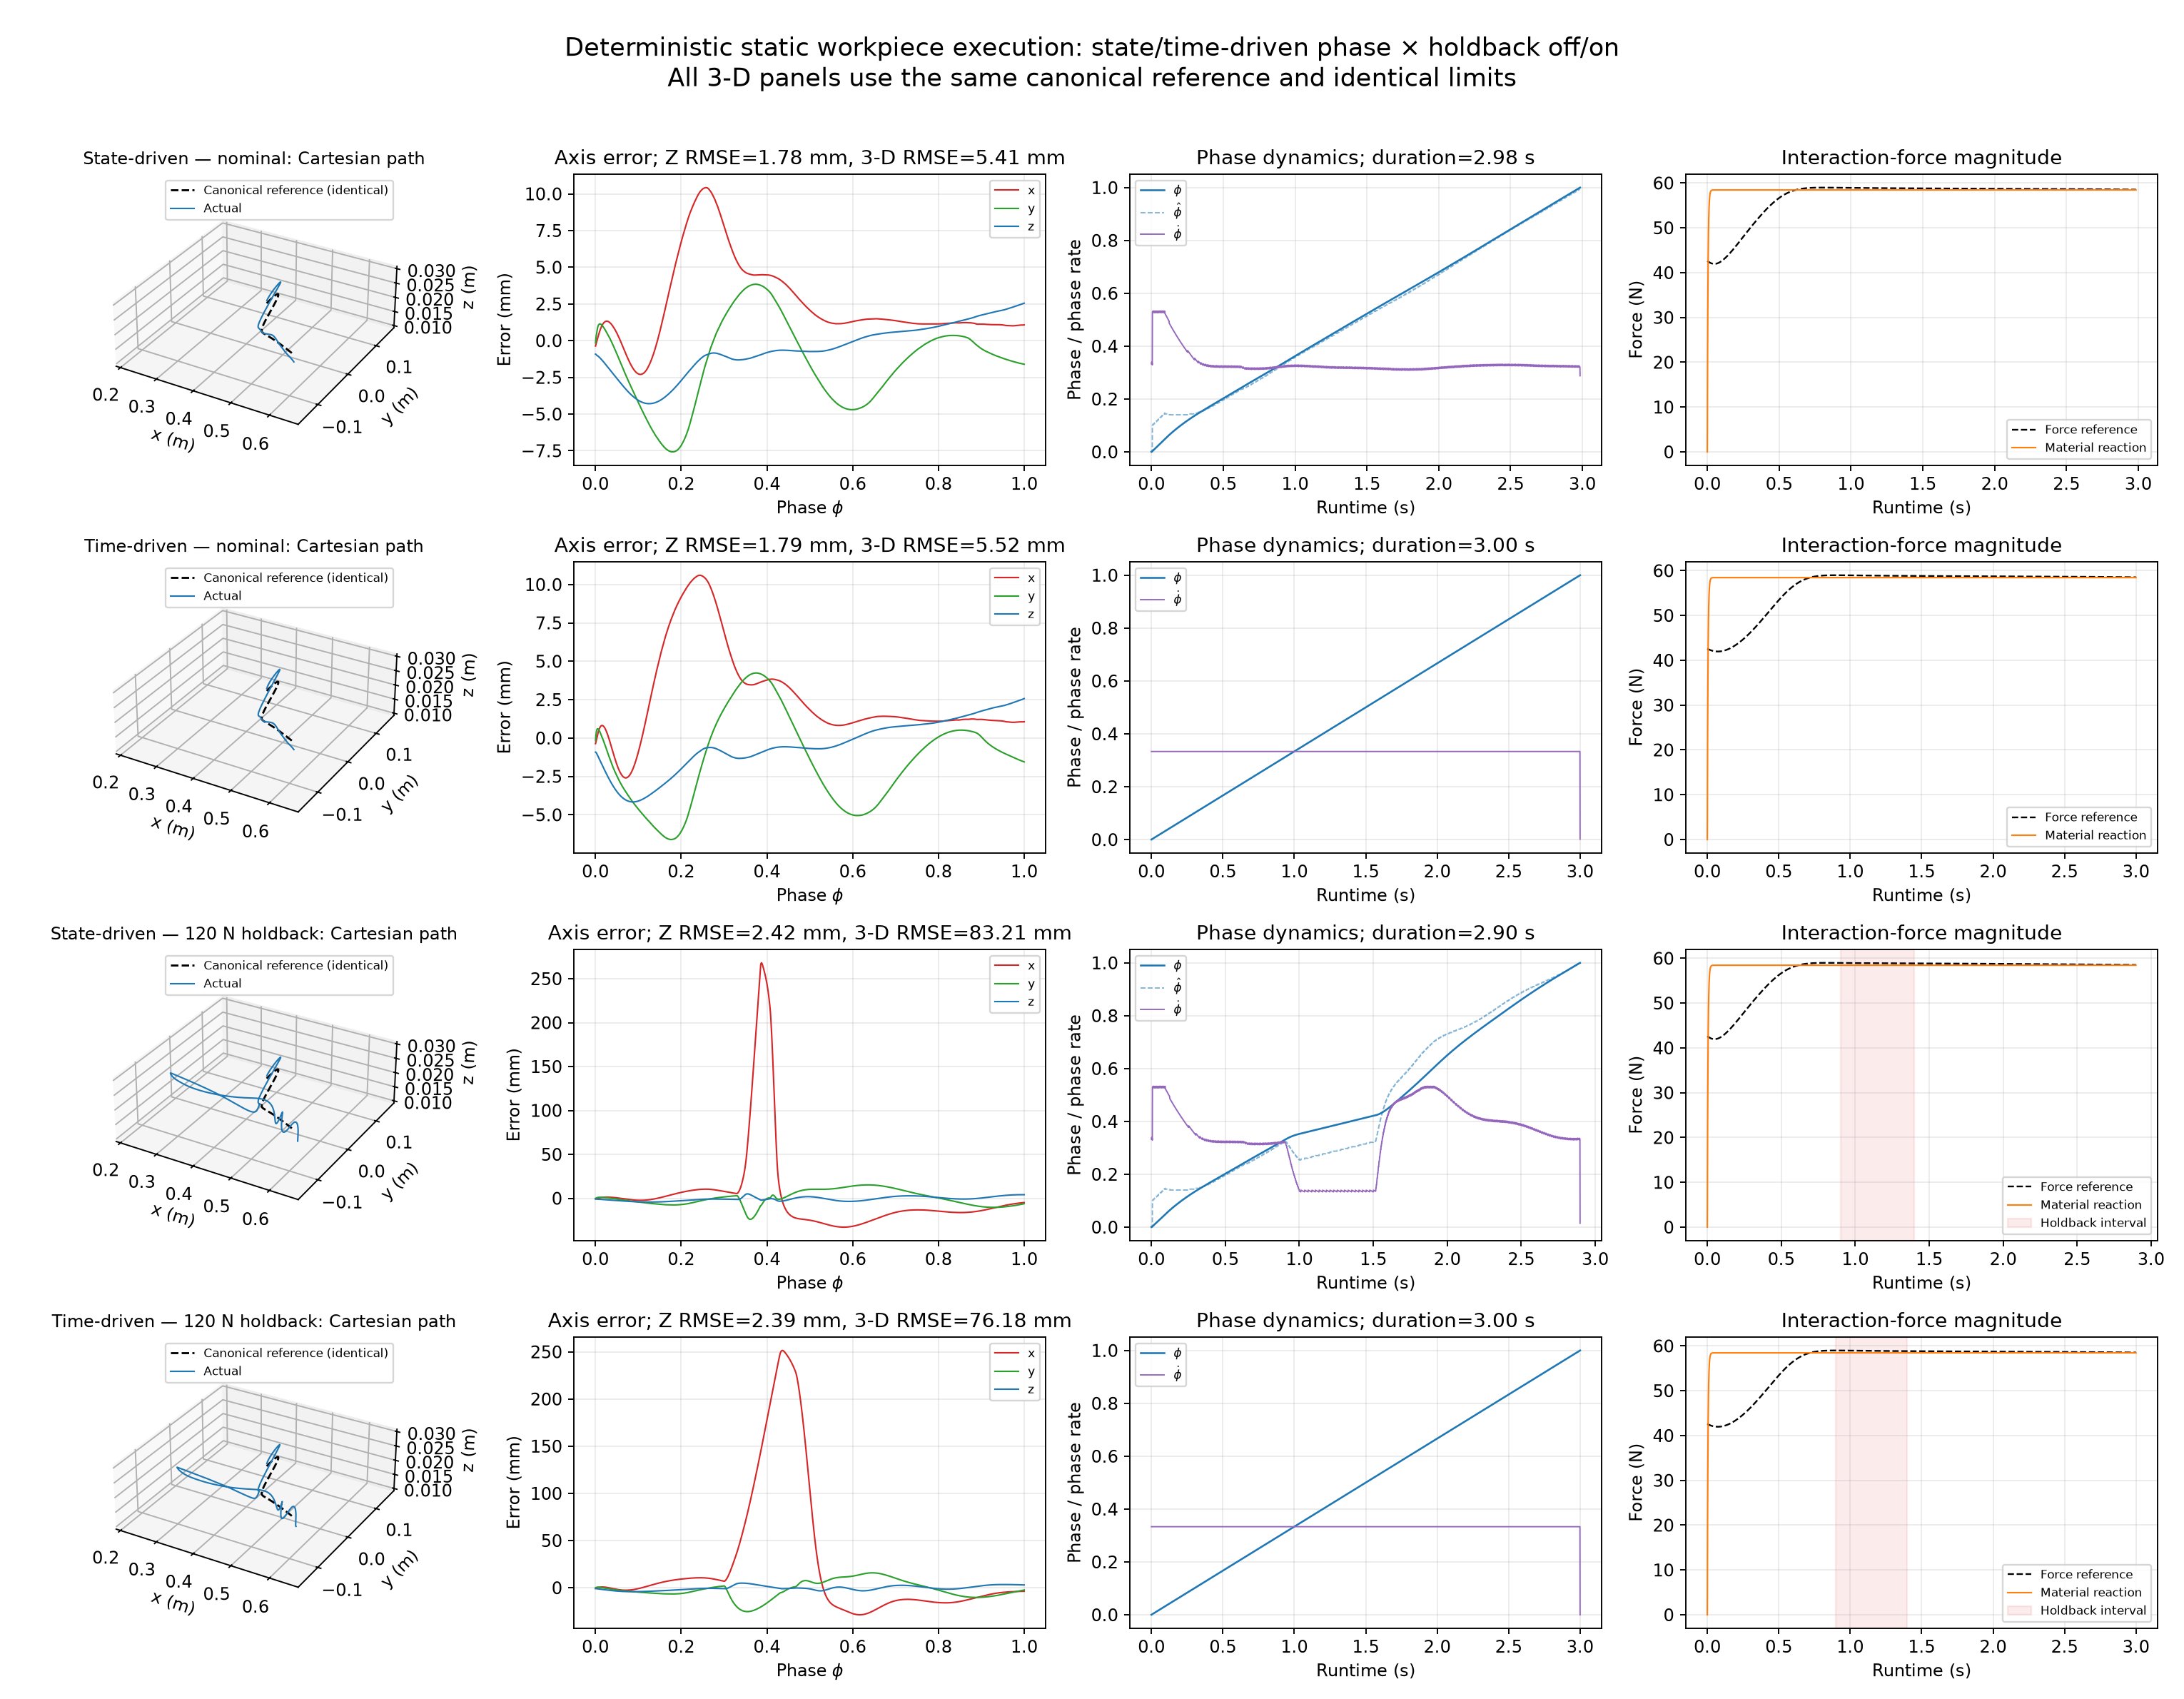
\includegraphics[width=\textwidth]{task_execution_four_case_static.png}
\caption{Deterministic static-workpiece execution without domain randomisation.
Rows cross state-driven/time-driven phase with holdback disabled/enabled;
columns show the Cartesian path, axis errors, phase dynamics and interaction
force. Every 3-D panel uses the same canonical geometric reference and identical
axis limits; only the executed trajectory changes. Nominal cut-depth RMSE is
$1.776$ and $1.791$\,mm for state- and time-driven execution, respectively.
Under holdback it is $2.424$ and $2.393$\,mm. The corresponding full Cartesian
RMSE increases to $83.208$ and $76.179$\,mm. Thus this 120\,N test demonstrates
constraint handling and phase response under a severe disturbance, not
high-accuracy rejection of that disturbance.}
\label{fig:execution_four_static}
\end{figure}

\begin{figure}[h]
\centering
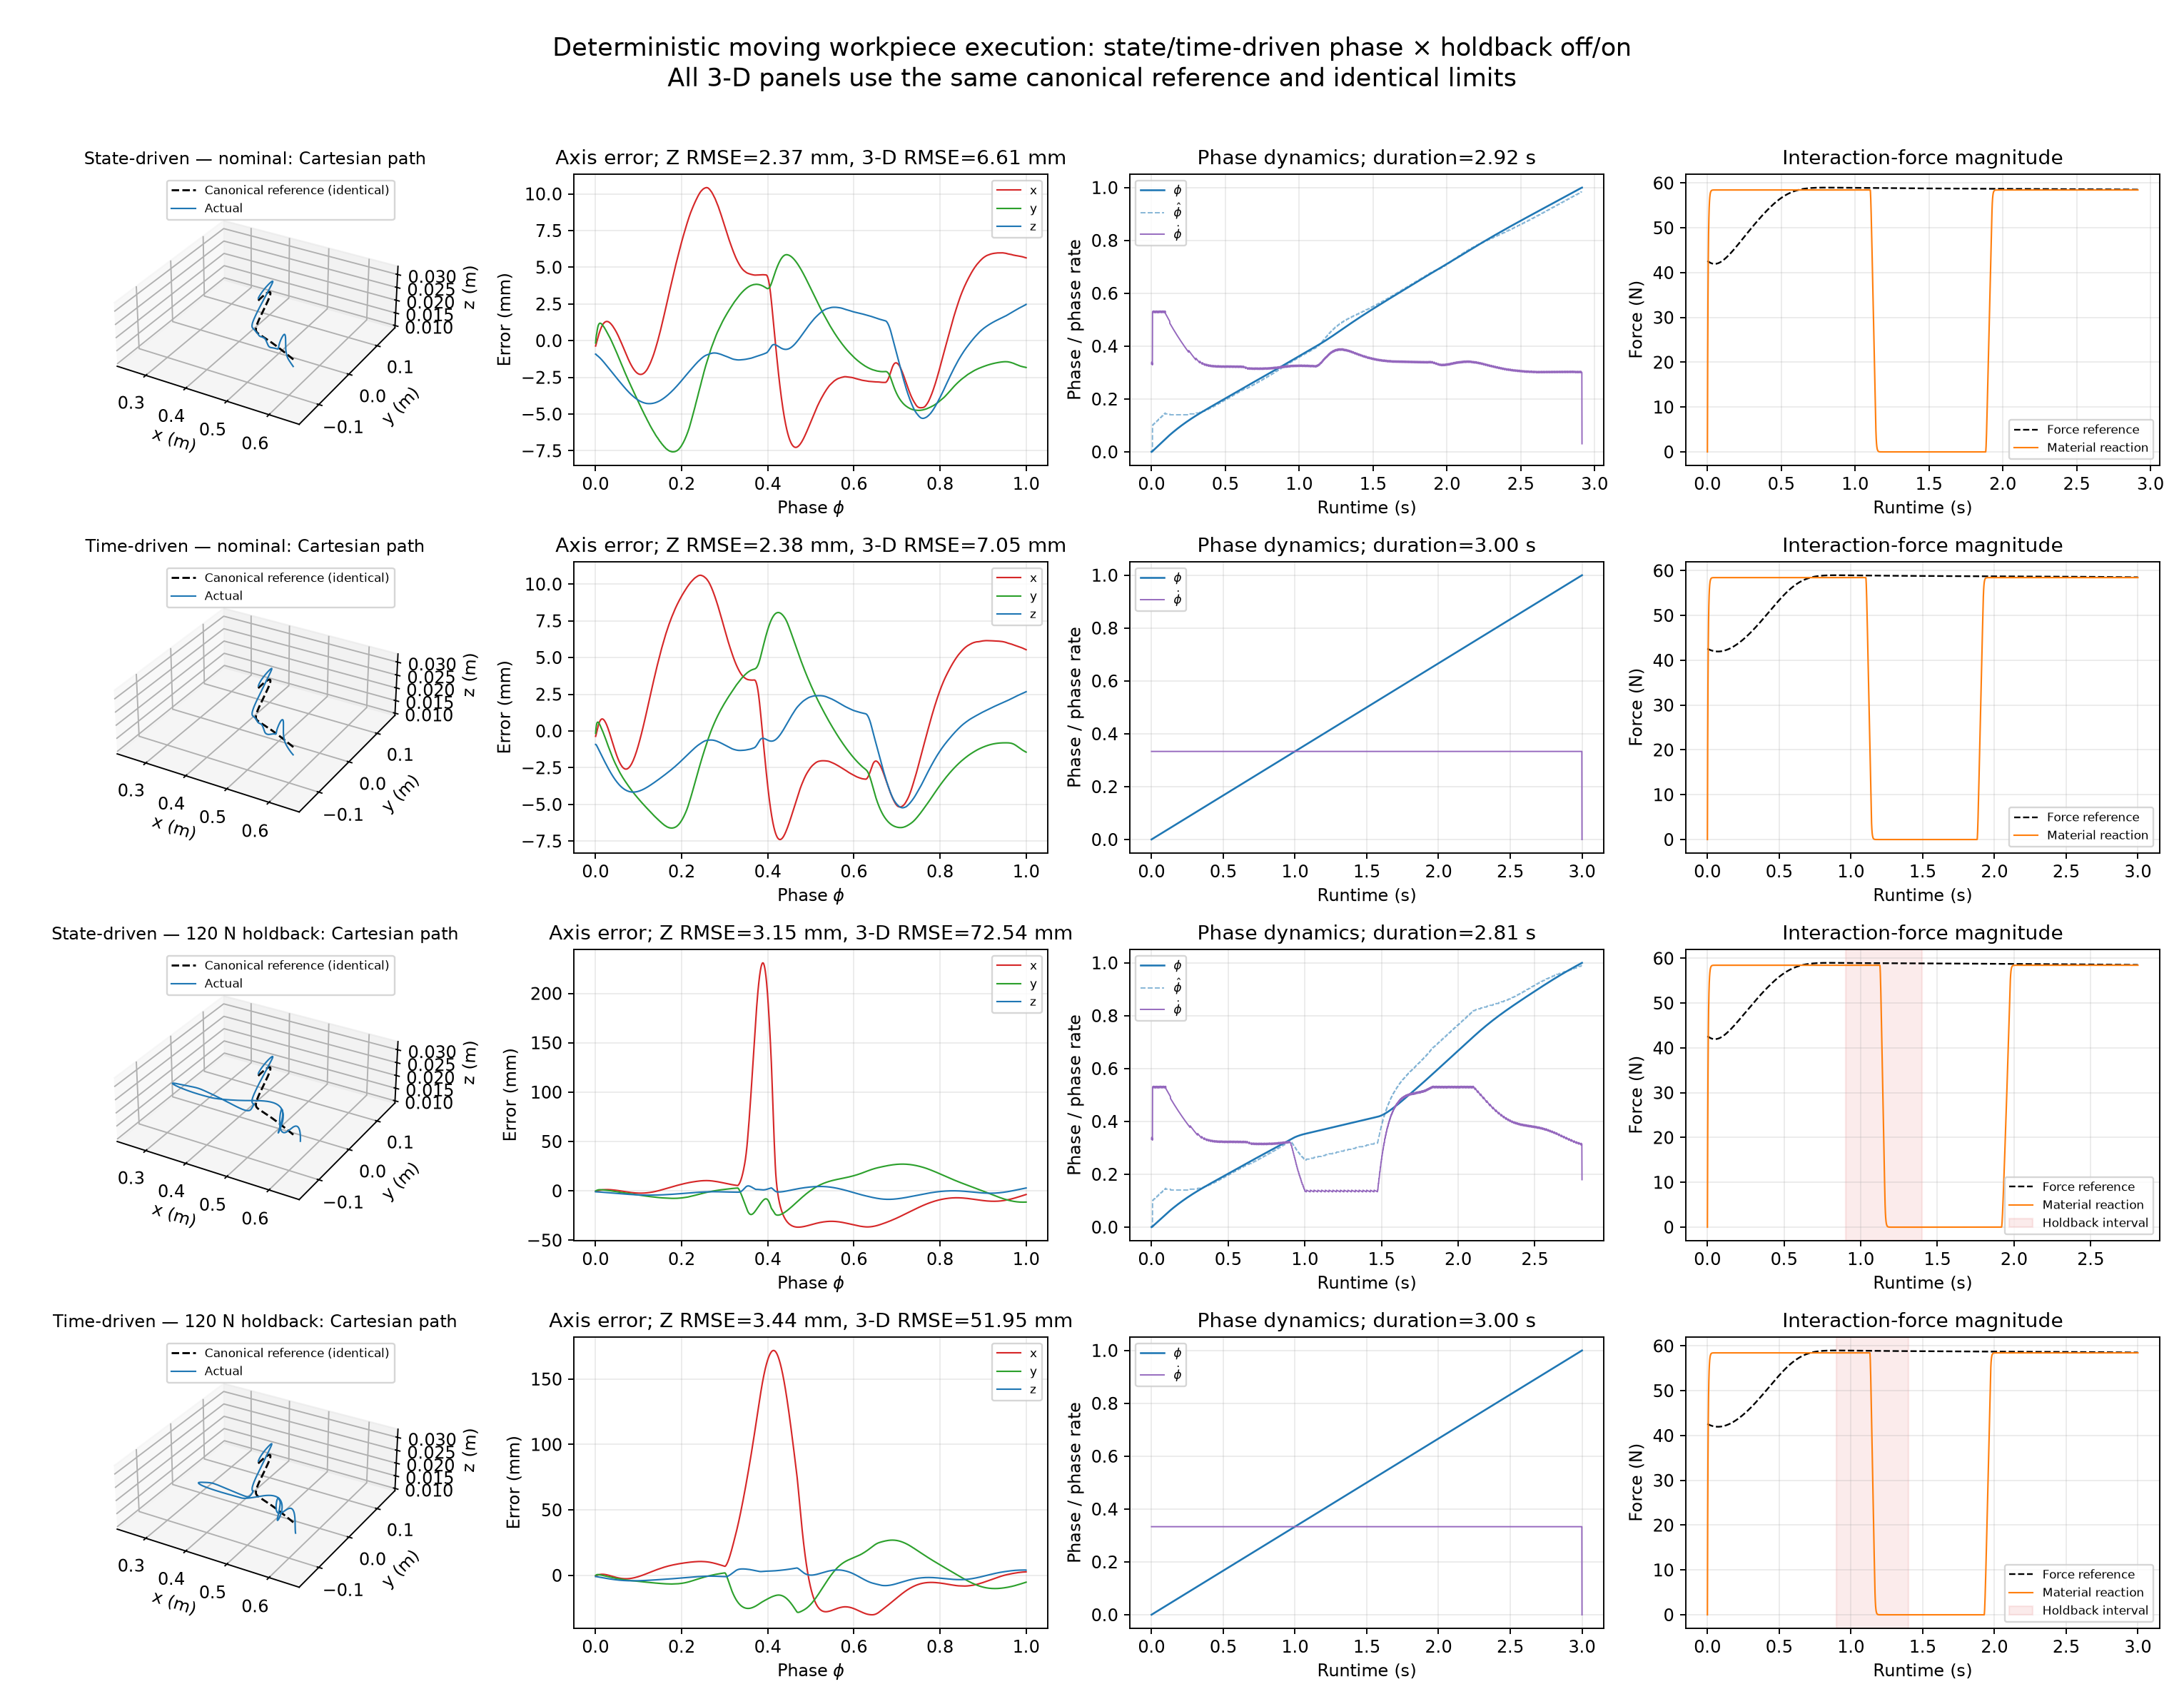
\includegraphics[width=\textwidth]{task_execution_four_case_moving.png}
\caption{Deterministic moving-workpiece execution under the same four
phase/holdback conditions as Fig.~\ref{fig:execution_four_static}. Nominal
cut-depth RMSE is $2.372$\,mm for state-driven timing and $2.384$\,mm for
time-driven timing. Under holdback the corresponding values are $3.148$ and
$3.442$\,mm, and full Cartesian RMSE is $72.541$ and $51.952$\,mm. Workpiece
motion changes only the environment geometry: it does not translate the
reference. Loss of contact can consequently occur when the material moves away
from the fixed commanded path.}
\label{fig:execution_four_moving}
\end{figure}

All $40$ executions completed and the torque-port power-violation fraction was
zero.  The state-driven law has slightly lower mean cut-depth RMSE in three
cells and is effectively equal in moving nominal execution. Full Cartesian
RMSE, however, is higher for state-driven timing in both moving-workpiece
cells. None of the paired cut-depth comparisons is significant
($p\in[0.4375,0.625]$). The large seed-to-seed dispersion, including a moving
workpiece outlier, precludes a general accuracy-improvement claim. The supported
result is narrower: state feedback changes phase progression while preserving
the implemented torque-port constraint and task completion. It does not reject
a 120\,N holdback with small Cartesian error, nor does it establish invariance
to workpiece motion.
Because learned precision-dependent impedance, the per-material cutting model,
force saturation, energy tank and torque projection remain active in every
cell, completion and constraint satisfaction evaluate the integrated proposed
architecture in both workpiece conditions.  The within-cell S--T difference,
by contrast, isolates only the incremental effect of state-dependent timing;
it must not be attributed to the other contributions.

% ============================================================================
\section{Conditional stability analysis and discrete torque-port energy accounting}
% ============================================================================
\label{sec:stab}
The scalpel obeys the task-space dynamics $\Lambda\ddot x+C\dot x+g=f+f_{\text{ext}}$, where $\Lambda\unit{kg}$ is
the Cartesian inertia and $f_{\text{ext}}\unit{N}$ the environment force.
Substituting the control law \eqref{eq:imp} (with gravity/Coriolis cancelled by
\eqref{eq:torque}) gives the \emph{error dynamics}
\begin{equation}
\Lambda\ddot{\tilde x}+\big(C+D(\phi)\big)\dot{\tilde x}+K(\phi)\,\tilde x=f_{\text{ext}} ,
\label{eq:err}
\end{equation}
a (time-varying) mass--spring--damper in the tracking error driven by the contact
force.

\subsection{Ideal continuous-time passivity condition}
\begin{proposition}[Continuous-time tank passivity under exact accounting]
\label{prop:pass}
At the Cartesian contact port, the input--output map
$f_{\text{ext}}\mapsto\dot x$ is passive under the following tank dynamics: With
the storage function (an energy, in joules)
$\mathcal S=\tfrac12\dot{\tilde x}^\top\Lambda\dot{\tilde x}+\tfrac12\tilde x^\top K\tilde x+T$
and a non-negative \emph{energy tank} $T\ge T_{\min}$ whose dynamics collect the
power dissipated by damping and compensate the power injected by the time-varying
gains and moving reference,
\begin{equation}
\dot T=\underbrace{\dot{\tilde x}^\top D\,\dot{\tilde x}}_{\text{collected }[\mathrm{W}]}
       -\underbrace{P_{\text{inj}}}_{[\mathrm{W}]},\qquad
P_{\text{inj}}=\tfrac12\tilde x^\top\dot K\,\tilde x+\tilde x^\top K\,\dot x_d ,
\end{equation}
the loop satisfies
$\dot{\mathcal S}\le f_{\text{ext}}^\top\dot x$ as long as $T>T_{\min}$.
\end{proposition}
\noindent Interpretation: $\mathcal S$ is the total stored energy (kinetic $+$ elastic $+$
tank). The two indefinite, potentially energy-injecting terms --- the rate of
change of stored elastic energy from a rising stiffness
($\tfrac12\tilde x^\top\dot K\tilde x$) and the power supplied to a moving
reference ($\tilde x^\top K\dot x_d$), both in watts --- are drawn from the tank,
which is recharged by the power dissipated through damping. When the tank
reaches its lower bound, stiffness growth is inhibited ($\dot K\!\le\!0$) and the
phase is frozen ($\dot\phi\!\to\!0$), so the controller cannot generate energy, instead,
it reduces the motion velocity to avoid instant change of dynamics.
This is an ideal continuous-time design condition. The implemented
sampled-data torque-port balance is stated separately below.

\subsection{Implemented discrete torque-port tank}
The simulation controller enforces the tank constraint at the joint torque port,
where the mechanical power supplied by the actuators is $P_\tau=\dot q^\top\tau$.
At every control step the nominal torque
\[
\tau_{\rm nom}=\tau_{\rm task}+\tau_{\rm null}+\tau_{\rm bias},
\qquad
\tau_{\rm task}=J^\top(JJ^\top+\lambda^2I)^{-1}f,
\qquad
\tau_{\rm null}=N\tau_{\rm posture},
\qquad
\tau_{\rm bias}=g+C\dot q
\]
is assembled from the task, null-space and model-compensation components.
The task torque $\tau_{\rm task}\unit{N\,m}$ maps the Cartesian impedance
command $f\unit{N}$ to the joints through the damped Jacobian inverse, where
$J\in\R^{3\times n}$ satisfies $\dot x=J\dot q$, $\lambda^2$ is the
damped-least-squares regulariser, $I$ is the identity matrix and $n$ is the
number of joints. The posture command $\tau_{\rm posture}\unit{N\,m}$ attracts
the arm towards its home configuration and damps joint motion. Its projection
$\tau_{\rm null}=N\tau_{\rm posture}$, with
$N=I-J^\top(JJ^\top+\lambda^2I)^{-1}J$, acts in the redundant null space and
therefore satisfies $JN\approx0$ without materially disturbing the Cartesian
cutting task. The bias term $\tau_{\rm bias}\unit{N\,m}$ contains the gravity
torque $g$ and the Coriolis/centrifugal torque $C\dot q$. Their sum
$\tau_{\rm nom}\unit{N\,m}$ is the nominal joint-torque command prior to
passivity enforcement.

The nominal command is projected onto the half-space of admissible torques:
\begin{equation}
\boxed{\;
\tau_{\rm safe}
=\arg\min_{\tau}\norm{\tau-\tau_{\rm nom}}_2^2
\quad\text{s.t.}\quad
\dot q^\top\tau \le P_{\max},\qquad
P_{\max}=\frac{T-T_{\min}}{h_c}. \;}
\label{eq:pass_qp}
\end{equation}
Here $\tau_{\rm safe}\unit{N\,m}$ is the projected actuator command,
$q\unit{rad}$ and $\dot q\unit{rad\,s^{-1}}$ are the joint position and
velocity, and $\dot q^\top\tau\unit{W}$ is the mechanical power supplied at the
joint port. The scalar $P_{\max}\unit{W}$ is the power available from the usable
tank energy $T-T_{\min}$ over one control period $h_c\unit{s}$.
Consequently, the constraint bounds positive energy delivery by the controller,
while negative joint power corresponds to energy absorption. The quadratic
objective retains the nominal control action as closely as possible in the
Euclidean torque norm. If
$\dot q^\top\tau_{\rm nom}\le P_{\max}$, then
$\tau_{\rm safe}=\tau_{\rm nom}$. Otherwise the Euclidean projection has the
closed form
\begin{equation}
\tau_{\rm safe}=\tau_{\rm nom}
-\frac{\dot q^\top\tau_{\rm nom}-P_{\max}}
       {\dot q^\top\dot q+\epsilon_\tau}\,\dot q ,
\label{eq:pass_projection}
\end{equation}
where $\epsilon_\tau>0$ is a small numerical regulariser. The correction lies
along $\dot q$, the direction that changes instantaneous joint power, and is
therefore the minimum-norm torque modification that satisfies the power bound.
This expression is also used as a fallback if the numerical QP does not return
a solution.

The power limit is computed from $T_k$, the torque is projected, and storage is
then settled from the delivered joint power:
\begin{equation}
P_k=\dot q_k^\top\tau_{{\rm safe},k},\qquad
T_{k+1}=\mathrm{clip}\!\left(T_k-h_cP_k,\,
T_{\min},T_{\max}\right),
\qquad
\gamma_{T,k+1}=\tanh\!\left(\frac{T_{k+1}-T_{\min}}{T_{\rm ref}}\right),
\label{eq:tank_disc}
\end{equation}
where $T_k\unit{J}$ and $T_{k+1}\unit{J}$ are the tank energies at consecutive
samples, $T_{\min}\unit{J}$ is the protected lower bound,
$T_{\max}\unit{J}$ is the storage ceiling, and $\mathrm{clip}(\cdot)$ enforces
these bounds. Positive commanded joint power depletes storage; negative power
recharges it, with excess absorbed energy discarded at $T_{\max}$. The
projection ensures $h_cP_k\le T_k-T_{\min}$ for positive $P_k$. The
implementation still logs damping, gain-variation and reference-motion powers
as diagnostics, but does not use them for a second tank update. The reference energy
$T_{\rm ref}\unit{J}$ sets the transition scale of the phase gate:
$\gamma_{T,k+1}\in[0,1]$ approaches zero as the usable tank energy
$T_{k+1}-T_{\min}$ vanishes and modulates the phase rate according to
$\dot\phi=\gamma_T\dot\phi_{\rm nom}$. Increasing $T_{\rm ref}$ makes this
transition more gradual over the available energy range.

The resulting closed-loop sequence couples the timing, impedance and
joint-torque layers.  At interval $k$, $T_k$ determines $\gamma_{T,k}$ and the
planned increment \eqref{eq:phase}; the current phase selects
$x_d$, $\dot x_d$, $K(\phi)$ and $D(\phi)$, from which the impedance law
produces $f$. The current tank determines $P_{\max}$, and the task mapping,
null-space term, dynamic compensation and projection produce
$\tau_{\rm safe}$ satisfying
$\dot q^\top\tau_{\rm safe}\le P_{\max}$. The delivered power then produces
$T_{k+1}$ and the next phase gate through \eqref{eq:tank_disc}. The nominal
experiments use $T_0=50$\,J, $T_{\max}=100$\,J and
$T_{\min}=0.001$\,J.

\begin{figure}[h]
\centering
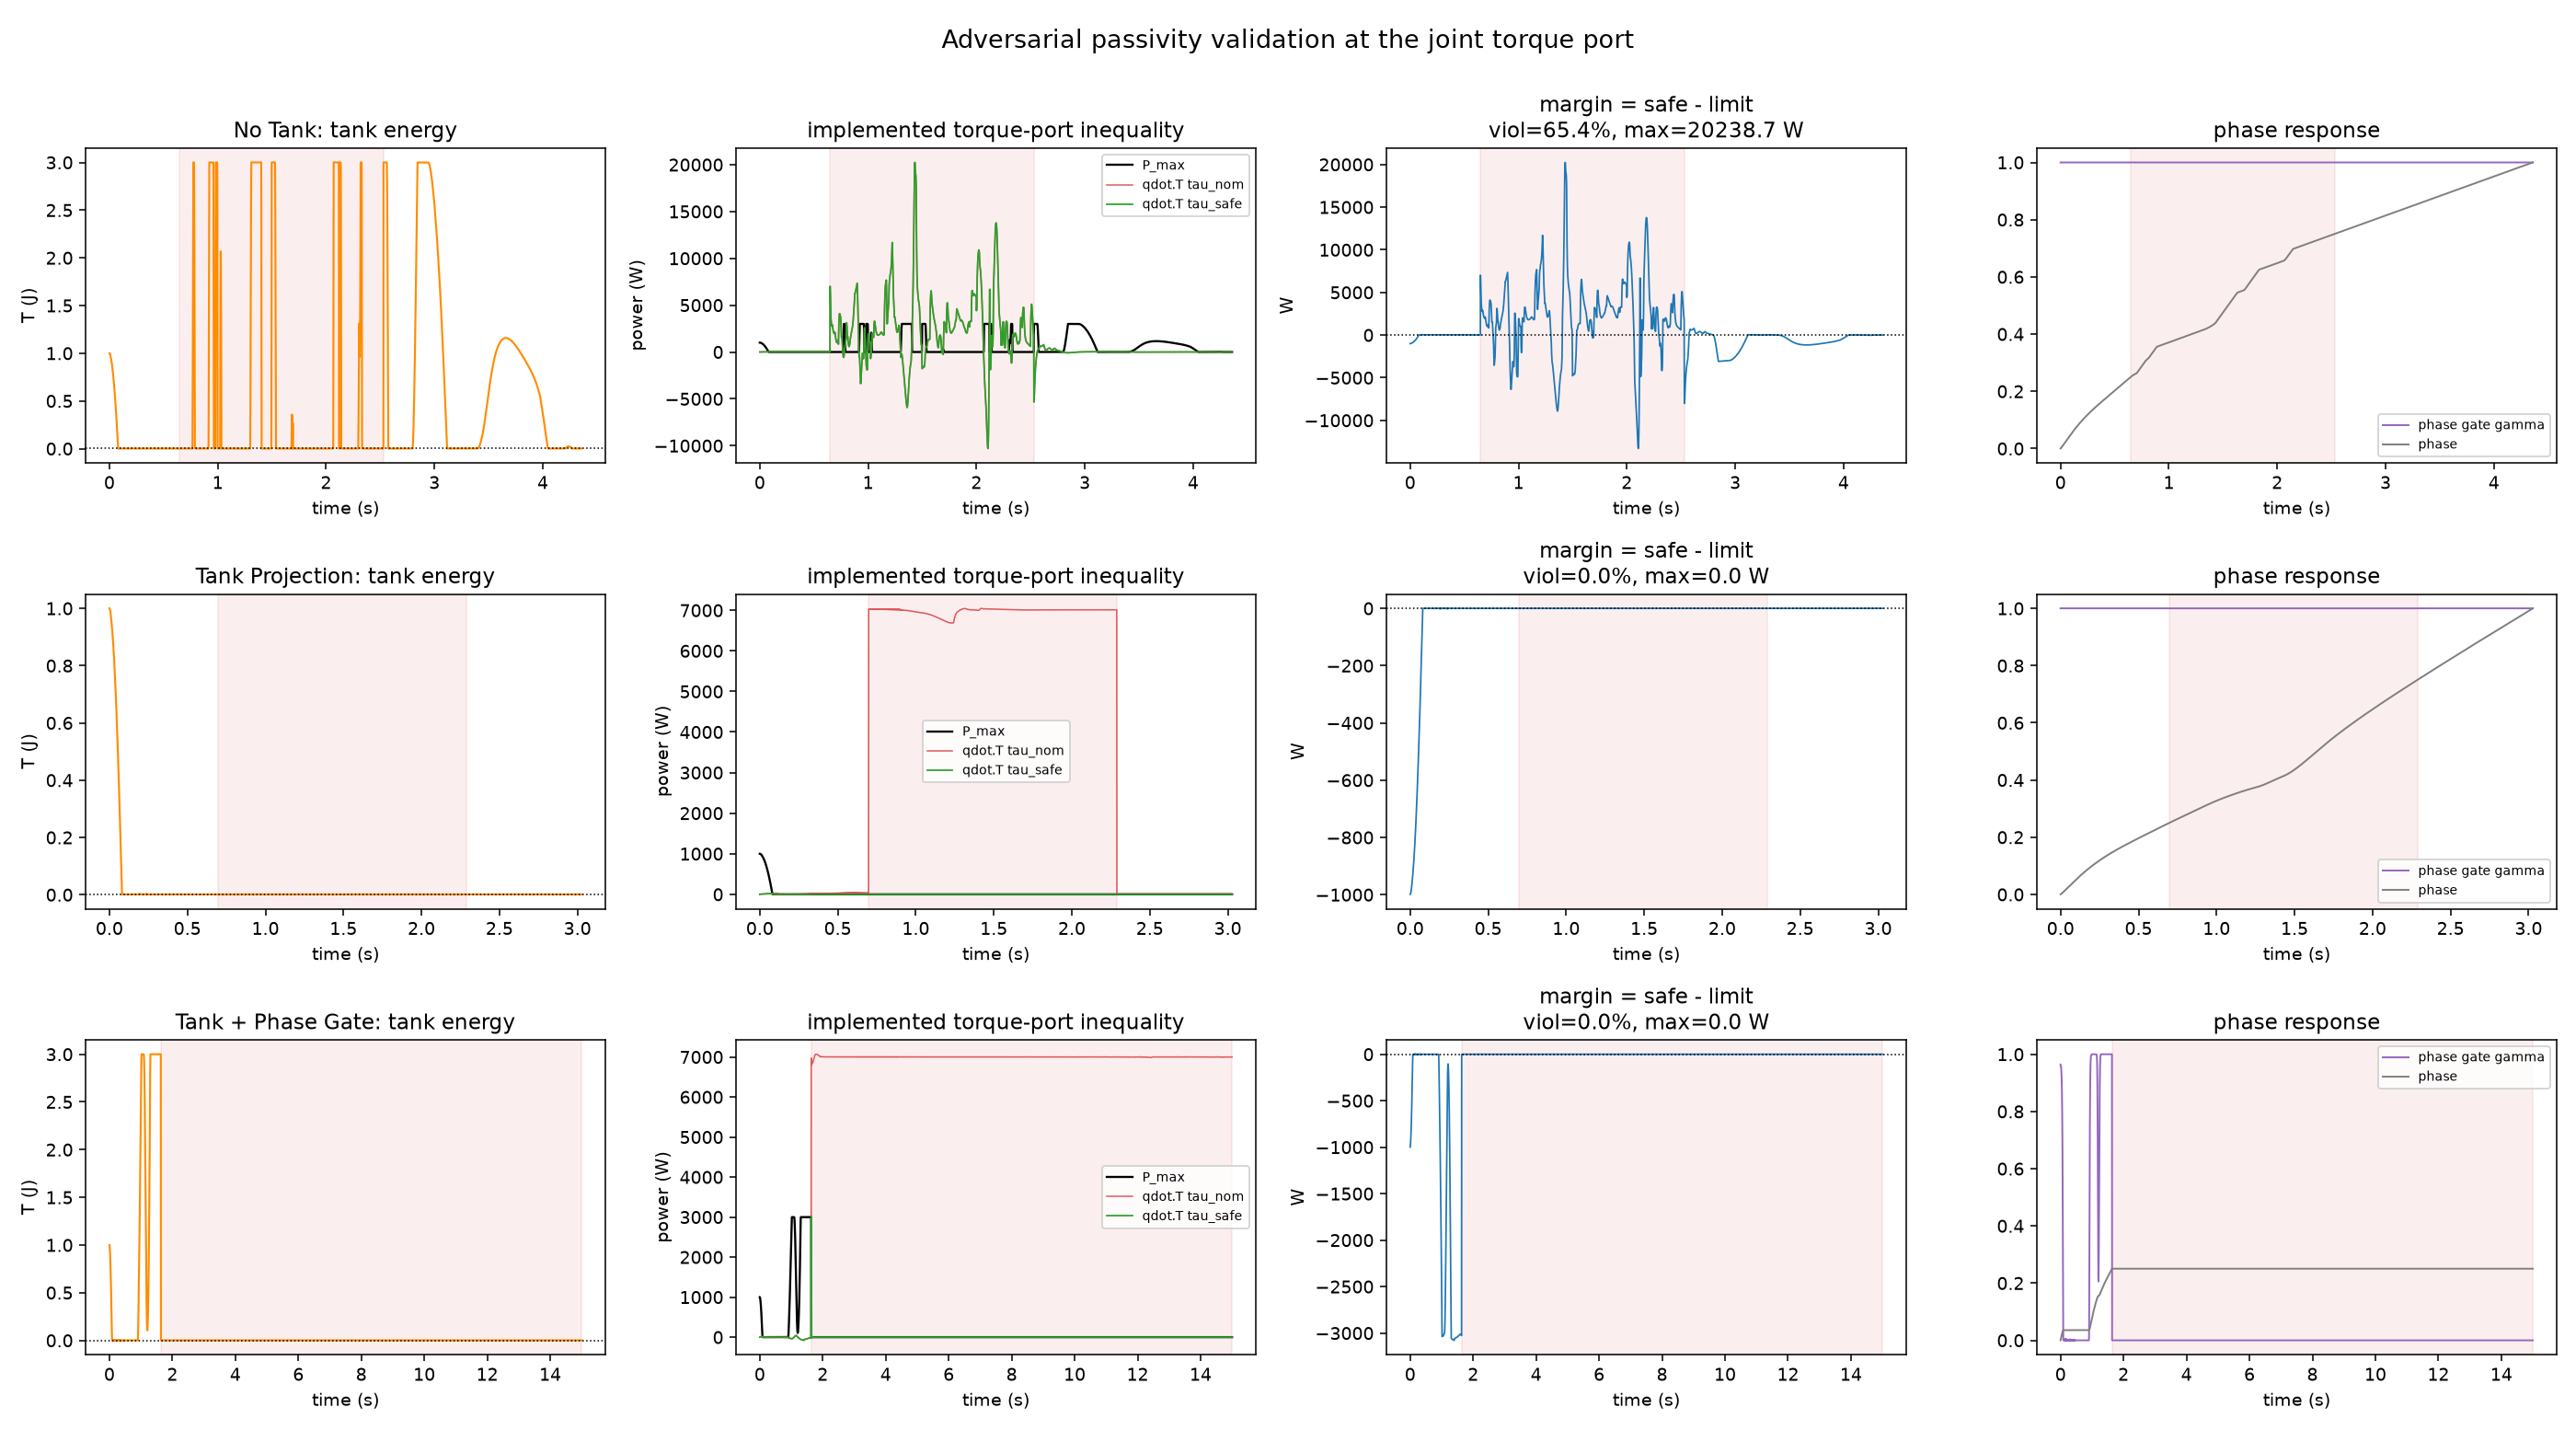
\includegraphics[width=0.97\textwidth]{passivity_adversarial_cork.png}
\caption{Positive-power perturbation validation on cork. A known positive joint-power
burst is injected before the torque projection. Without projection (top row),
$\dot q^\top\tau$ exceeds the counterfactual budget for $65.4\%$ of samples
and reaches a maximum margin of $+20{,}239$\,W. With torque projection
(middle and bottom), the implemented inequality
$\dot q^\top\tau_{\rm safe}-P_{\max}\le0$ has $0.0\%$ logged violations.
With the deliberately small $1$\,J validation tank, phase gating stops progress
at $\phi=0.25$ after storage depletion; safety intervention therefore does not
imply task completion.}
\label{fig:pass_adv}
\end{figure}

\begin{table}[h]
\centering
\begin{tabular}{lcccc}
\toprule
Controller & completion & min. tank (J) & budget violation & max margin (W)\\
\midrule
No projection & $100\%$ & $0.001$ & $65.4\%$ & $+20{,}239$\\
Tank projection & $100\%$ & $0.001$ & $0.0\%$ & $0$\\
Tank + phase gate & $0\%$ ($\phi_f=0.25$) & $0.001$ & $0.0\%$ & $0$\\
\bottomrule
\end{tabular}
\caption{Torque-port storage and power validation under positive-power
injection. Projection enforces the sampled bound. With phase gating and the
stress-test's $1$\,J tank, depleted storage halts the task rather than violating
the bound.}
\label{tab:pass_adv}
\end{table}

This is an empirical validation of the implemented sampled storage and power
accounting, not a universal passivity or completion proof. The
reconstructed Cartesian residual $\dot V-f_{\text{ext}}^\top\dot x$ is still
plotted as a diagnostic in Fig.~\ref{fig:stab}, but it depends on finite
differences, force-estimator sign conventions and an approximate Cartesian
inertia; the implemented guarantee is therefore stated and validated at the
torque port $\dot q^\top\tau$.

\subsection{Sufficient exponential-stability conditions for idealised error dynamics}
The stability argument is first established for nominal regulation and is then
extended to phase-varying gains and bounded perturbations.

\begin{assumption}[Nominal regulation conditions]
\label{ass:nominal_stability}
The compensated Cartesian inertia satisfies
$\Lambda=\Lambda^\top\succ0$ and is constant over the local analysis interval;
the frozen gains satisfy $K=K^\top\succ0$ and $D=D^\top\succ0$; gravity and
Coriolis terms are compensated; and the nominal result is evaluated with zero
external input and zero unmodelled reference acceleration.
\end{assumption}

Under Assumption~\ref{ass:nominal_stability}, defining
$e=\tilde x$, $v=\dot{\tilde x}$ and
$z=[e^\top\;v^\top]^\top$, the error system becomes
\begin{equation}
\dot z=A z,\qquad
A=
\begin{bmatrix}
0&I\\
-\Lambda^{-1}K&-\Lambda^{-1}D
\end{bmatrix}.
\label{eq:error_state}
\end{equation}
The matrix $\Lambda\unit{kg}$ is the Cartesian inertia,
$K\unit{N\,m^{-1}}$ and $D\unit{N\,s\,m^{-1}}$ are the frozen stiffness and
damping matrices, and $A$ is the corresponding state matrix. The mechanical
energy
$V_0=\tfrac12v^\top\Lambda v+\tfrac12e^\top K e$ satisfies only
$\dot V_0=-v^\top Dv\le0$. A strict decay rate in both $e$ and $v$ is obtained
by adding a position--velocity cross-term:
\begin{equation}
V(z)=\tfrac12v^\top\Lambda v+\tfrac12e^\top K e
 +\beta e^\top\Lambda v
 =\tfrac12z^\top Pz,\qquad
P=
\begin{bmatrix}
K&\beta\Lambda\\
\beta\Lambda&\Lambda
\end{bmatrix},\qquad\beta>0 .
\label{eq:lyap}
\end{equation}
Here $\beta\unit{s^{-1}}$ weights the cross-term. By the Schur complement,
\begin{equation}
P\succ0
\quad\Longleftrightarrow\quad
K-\beta^2\Lambda\succ0,
\label{eq:P_condition}
\end{equation}
for which the scalar condition
$\beta^2<\lambda_{\min}(K)/\lambda_{\max}(\Lambda)$ is sufficient. Hence,
with $\underline p=\lambda_{\min}(P)$ and
$\overline p=\lambda_{\max}(P)$,
\begin{equation}
\frac{\underline p}{2}\norm{z}^2
\le V(z)\le
\frac{\overline p}{2}\norm{z}^2 .
\label{eq:V_bounds}
\end{equation}

\begin{theorem}[Exponential stability]
\label{thm:exp}
For the nominal system \eqref{eq:error_state}, suppose $P\succ0$ and
\begin{equation}
\begin{split}
Q&=
\begin{bmatrix}
2\beta K&\beta D\\
\beta D&2(D-\beta\Lambda)
\end{bmatrix}\succ0 .
\end{split}
\label{eq:Q_condition}
\end{equation}
Then the origin $z=0$ is globally exponentially stable. In particular, with
$\underline q=\lambda_{\min}(Q)$,
\begin{equation}
\dot V\le-\alpha V,\qquad
\alpha=\frac{\underline q}{\overline p},
\qquad
\norm{z(t)}
\le
\sqrt{\frac{\overline p}{\underline p}}\,
e^{-\alpha t/2}\norm{z(0)} .
\label{eq:exp_bound}
\end{equation}
\end{theorem}
\begin{proof}
Using $\Lambda\dot v=-Dv-Ke$, differentiation of \eqref{eq:lyap} gives
\begin{align}
\dot V
&=v^\top\Lambda\dot v+e^\top Kv
  +\beta v^\top\Lambda v+\beta e^\top\Lambda\dot v \nonumber\\
&=-v^\top(D-\beta\Lambda)v-\beta e^\top Ke-\beta e^\top Dv
 =-\tfrac12z^\top Qz .
\label{eq:V_derivative}
\end{align}
The cancellation of $-v^\top Ke+e^\top Kv$ removes the conservative
spring-power exchange. From $Q\succ0$ and \eqref{eq:V_bounds},
\[
\dot V\le-\frac{\underline q}{2}\norm{z}^2
\le-\frac{\underline q}{\overline p}V=-\alpha V.
\]
Integration gives $V(t)\le e^{-\alpha t}V(0)$, and substitution of the upper
and lower quadratic bounds in \eqref{eq:V_bounds} yields
\eqref{eq:exp_bound}.
\end{proof}

Condition \eqref{eq:Q_condition} can be checked directly from the learned gains
and Cartesian inertia at each phase. Its Schur-complement form,
\begin{equation}
D-\beta\Lambda-\frac{\beta}{4}DK^{-1}D\succ0,
\label{eq:Q_schur}
\end{equation}
also shows why $D-\beta\Lambda\succ0$ alone is insufficient: the mixed term
$-\beta e^\top Dv$ must also be dominated. The computable rate
$\alpha=\lambda_{\min}(Q)/\lambda_{\max}(P)$ expresses the joint influence of
inertia, stiffness, damping and the selected cross-term coefficient.

\begin{figure}[h]
\centering
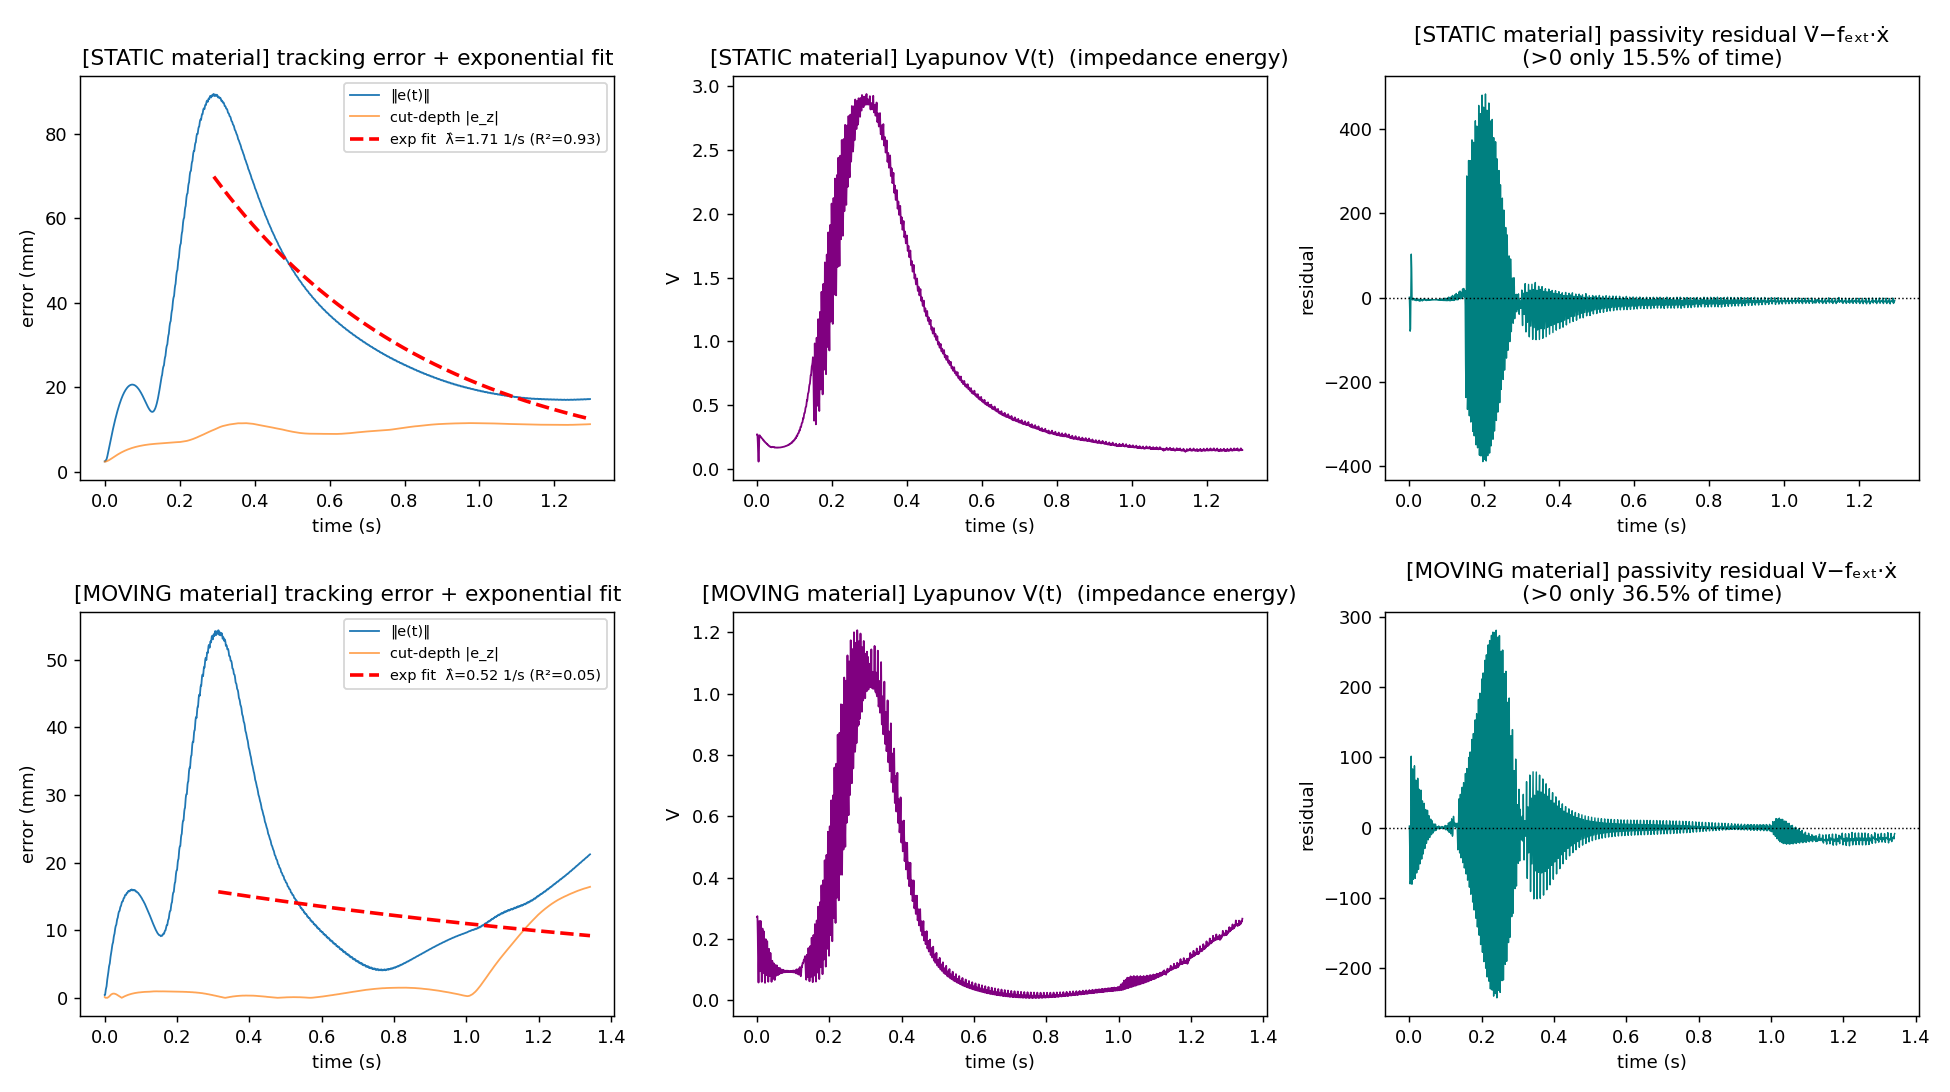
\includegraphics[width=0.97\textwidth]{stability_cork.png}
\caption{Nominal stability and passivity diagnostics on cork. The left column
shows tracking error and cut-depth error; the middle column shows the Lyapunov
diagnostic and tank energy; the third column shows the implemented torque power
budget $P_{\max}$ together with nominal and projected torque power; the right
column shows the reconstructed Cartesian residual, used as a diagnostic rather
than as the primary passivity proof.}
\label{fig:stab}
\end{figure}

\paragraph{Time-varying gains and moving-reference perturbations.}
For $K=K(\phi)$, $D=D(\phi)$ and an aggregated Cartesian perturbation
$\delta$ containing external contact input, imperfect model compensation and
uncompensated reference acceleration, the derivative becomes
\begin{equation}
\dot V
=-\tfrac12z^\top Q(\phi)z
+\tfrac12e^\top\dot K(\phi)e
+(v+\beta e)^\top\delta,
\qquad
\dot K(\phi)=K'(\phi)\dot\phi .
\label{eq:V_varying}
\end{equation}

\begin{corollary}[Uniform exponential stability with variable gains]
\label{cor:variable_exp}
Suppose $P(\phi)\succ0$ and $Q(\phi)\succ0$ uniformly for
$\phi\in[0,1]$, and define
\begin{equation}
q_*=\inf_{\phi\in[0,1]}\lambda_{\min}\!\big(Q(\phi)\big),\qquad
\kappa=\sup_{\phi\in[0,1]}\norm{\dot K(\phi)}_2,\qquad
\mu=q_*-\kappa .
\label{eq:uniform_margin}
\end{equation}
If $\mu>0$, the unforced time-varying system is uniformly exponentially stable.
Since
$\norm{\dot K(\phi)}_2\le\norm{K'(\phi)}_2|\dot\phi|$, a sufficient phase-rate
condition is
\begin{equation}
|\dot\phi|
<
\frac{q_*}{{\displaystyle
\sup_{\phi\in[0,1]}\norm{K'(\phi)}_2}} .
\label{eq:phase_stability_bound}
\end{equation}
\end{corollary}
\begin{proof}
With $\delta=0$, equations~\eqref{eq:V_varying} and
\eqref{eq:uniform_margin} give
\[
\dot V\le-\tfrac12\big(q_*-\kappa\big)\norm{z}^2
=-\tfrac12\mu\norm{z}^2.
\]
Uniform positive lower and upper bounds on $P(\phi)$ imply exponential decay by
the comparison argument used in Theorem~\ref{thm:exp}.
Condition~\eqref{eq:phase_stability_bound} ensures $\kappa<q_*$ and therefore
$\mu>0$.
\end{proof}

The tank gate \eqref{eq:tank_disc} reduces $\dot\phi$ as usable energy
decreases and therefore reduces $\dot K$ and the moving-reference power demand.
The torque projection \eqref{eq:pass_qp} independently enforces the joint-port
power constraint. Passivity follows from the energy accounting, whereas
uniform exponential stability additionally requires the matrix margin
\eqref{eq:uniform_margin}; the two properties are related through phase gating
but are not identical claims.

\begin{proposition}[Practical exponential stability under bounded perturbations]
\label{prop:practical_exp}
Let the conditions of Corollary~\ref{cor:variable_exp} hold, define
$g_\beta=\sqrt{1+\beta^2}$, and suppose that
$\sup_{s\ge0}\norm{\delta(s)}<\infty$. Then
\begin{equation}
\dot V
\le-\frac{\mu}{4}\norm{z}^2
+\frac{g_\beta^2}{\mu}\norm{\delta}^2
\le-aV+\frac{g_\beta^2}{\mu}\norm{\delta}^2,
\qquad
a=\frac{\mu}{2\overline p},
\label{eq:ISS_derivative}
\end{equation}
where $\overline p=\sup_\phi\lambda_{\max}(P(\phi))$. Integration gives
\begin{equation}
V(t)\le e^{-at}V(0)
+\frac{g_\beta^2}{a\mu}
 \left(1-e^{-at}\right)
 \sup_{0\le s\le t}\norm{\delta(s)}^2 .
\label{eq:ISS_bound}
\end{equation}
Accordingly, the state converges exponentially to a residual set whose radius
is proportional to $\sup\norm{\delta}$; when $\delta=0$, this set collapses to
the origin.
\end{proposition}
\begin{proof}
The perturbation term in \eqref{eq:V_varying} satisfies
$|(v+\beta e)^\top\delta|
\le g_\beta\norm{z}\norm{\delta}$. Young's inequality with the uniform margin
$\mu$ yields \eqref{eq:ISS_derivative}; integration of the scalar differential
inequality gives \eqref{eq:ISS_bound}.
\end{proof}

\paragraph{Experimental interpretation.}
Theorem~\ref{thm:exp} provides the frozen-gain nominal result,
Corollary~\ref{cor:variable_exp} states the uniform margin required while the
learned gains evolve with phase, and Proposition~\ref{prop:practical_exp}
accounts for bounded workpiece motion, contact forces and compensation error.
Figure~\ref{fig:stab} reports the corresponding empirical diagnostics. The
logged cut-depth error and storage remain bounded in the plotted episodes. The fitted decay
of the full Cartesian error is interpreted cautiously because low-precision
axes are intentionally assigned low stiffness and therefore have smaller
contraction margins.

\paragraph{Implementation status.} The live tank state determines the
torque-level budget in \eqref{eq:pass_qp}, while phase progression is gated by
\eqref{eq:tank_disc}. The positive-power perturbation validation in
Fig.~\ref{fig:pass_adv} and Table~\ref{tab:pass_adv} evaluate the implemented
storage and torque-power constraints. Equations~\eqref{eq:Q_condition}--\eqref{eq:ISS_bound}
separately state nominal, uniform time-varying and perturbed sufficient
conditions. The runtime does not calculate $P(\phi)$, $Q(\phi)$, $q_*$ or
$\mu$; the plots therefore diagnose boundedness but do not verify the matrix
conditions of the theorems.

% ============================================================================
\section{Material interaction model}
% ============================================================================
\label{sec:material}
In simulation the controller tracked position well, yet the contact force at first
failed to match the demonstrated force. The stock simulated \emph{material model}
presents both the scalpel blade and the workpiece as rigid box geometries; hence,
overlapping boxes in a rigid-contact simulator produce solver-dependent
\emph{collision forces}, unlike the physical nature of the real cutting force.
Their magnitude is set by contact penetration, time step and solver parameters,
and their direction by the instantaneous collision normal. A controller cannot
make such a contact respect a demonstrated cutting
law, because the measured ``force'' is a geometric contact artefact rather than a
material-specific \emph{fracture force}. Figure~\ref{fig:before_after} shows this
failure mode in a matched comparison: the same controller, trajectory, gains and
cork workpiece are used, and only the contact model is toggled.

\begin{proposition}[Why box-on-box contact is not a cutting model]
Let the desired cutting interaction be a material law
$F_d(\phi)=\bar F(d(\phi))\,r(\phi)$ with bounded magnitude
$0\le\bar F(d)\le F_{\rm mat}^{\rm cut}$ and unit reaction direction
$r(\phi)$ learned from the demonstration. A rigid box-on-box MuJoCo contact
generates instead
\begin{equation}
F_{\rm box}=F_{\rm solver}(q,\dot q,h_{\rm sim},\texttt{solref},\texttt{solimp},
                          \mathcal C(q),\mu_c),
\label{eq:box_solver}
\end{equation}
where $h_{\rm sim}$ is the simulator integration step,
$\mathcal C(q)$ is the active contact set and
$\mu_c$ denotes the friction parameters. In general there exists no
depth-only map $\mathcal F:\R_{\ge0}\rightarrow\R^3$ that is invariant to these
numerical and geometric quantities and satisfies simultaneously
$F_{\rm box}=\mathcal F(d)=\bar F(d)r(\phi)$ along the demonstrated cut.
\end{proposition}

\begin{proof}
Assume such an invariant $\mathcal F(d)$ exists. Consider two simulator
configurations with the same blade pose and hence the same penetration $d$, but
with distinct solver settings
$\vartheta_1=(h_{{\rm sim},1},\texttt{solref}_1,\texttt{solimp}_1)$ and
$\vartheta_2=(h_{{\rm sim},2},\texttt{solref}_2,\texttt{solimp}_2)$. The normal reaction in a
penalty or constraint-regularised contact has the generic dependence
\begin{equation}
F_{n,i}=\Psi(d,\dot d;\vartheta_i),\qquad i\in\{1,2\},
\label{eq:solver_dependence}
\end{equation}
and changing the effective contact stiffness, damping or discrete step gives
$\Psi(d,\dot d;\vartheta_1)\ne\Psi(d,\dot d;\vartheta_2)$ for some
$(d,\dot d)$. Thus identical $d$ produces different force magnitudes, which
contradicts the assumed depth-only invariance.

Independently, the rigid-contact force satisfies the friction-cone restriction
\begin{equation}
F_{\rm box}=F_n n_c+F_t,\qquad
F_n\ge0,\quad n_c^\top F_t=0,\quad
\norm{F_t}\le\mu_cF_n ,
\label{eq:friction_cone}
\end{equation}
where $n_c$ is a normal selected by the active box feature. At a face or edge
transition, $\mathcal C(q)$ and $n_c$ can change while $d$ remains continuous.
The resulting force direction is therefore determined by collision geometry
and need not equal the demonstrated $r(\phi)$. Since equality with the cutting
law requires both
\[
\norm{F_{\rm box}}=\bar F(d)
\quad\text{and}\quad
\frac{F_{\rm box}}{\norm{F_{\rm box}}}=r(\phi),
\]
failure of either condition disproves
$F_{\rm box}=\bar F(d)r(\phi)$. Hence the rigid collision map cannot supply the
missing material-specific constitutive relation.
\end{proof}

\begin{figure}[h]
\centering
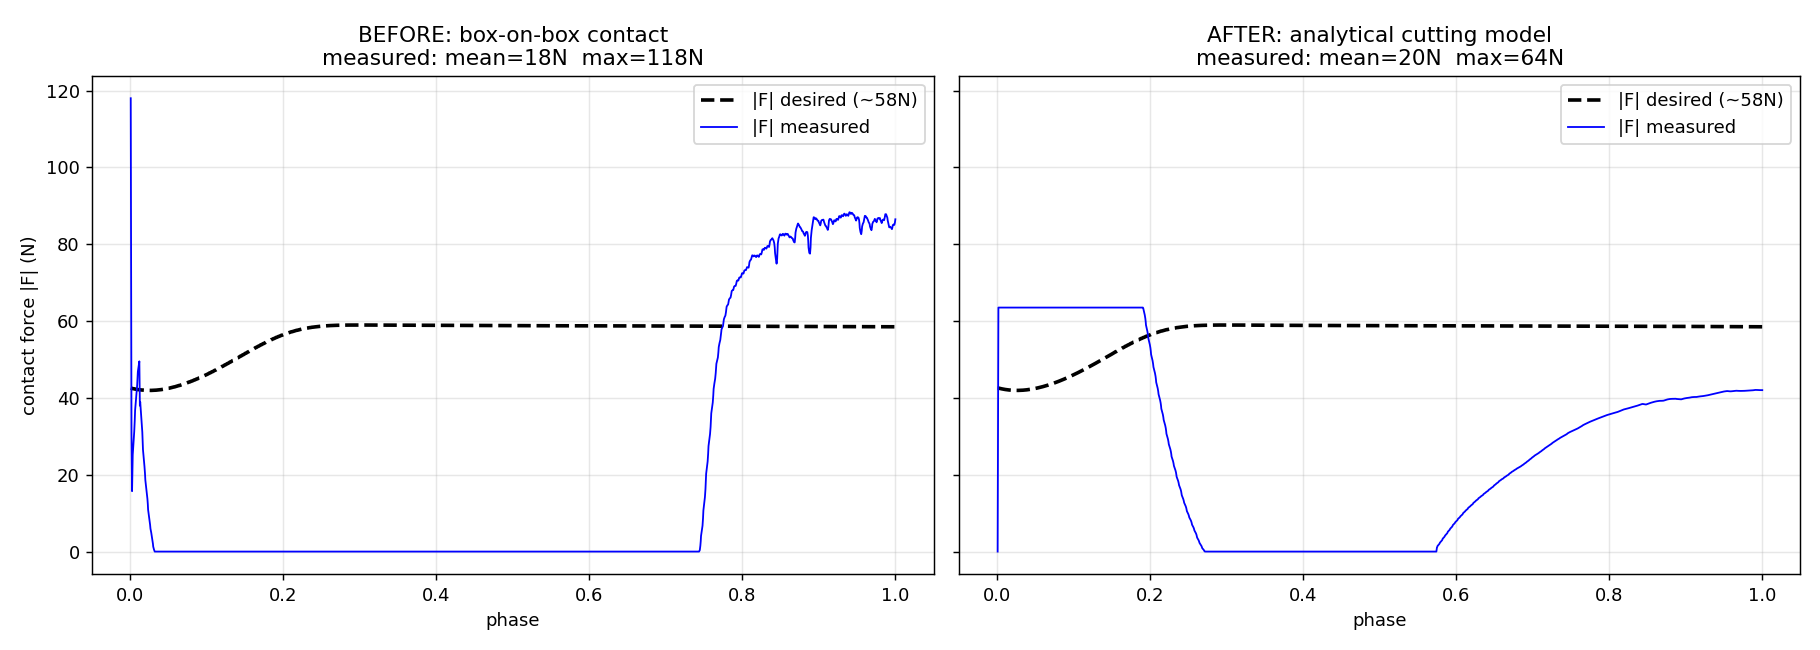
\includegraphics[width=0.97\textwidth]{cutting_model_fix.png}
\caption{Why a material model is needed. This matched cork comparison uses the same
controller and toggles only the contact physics. Top row: rigid box-on-box
contact over-reacts and follows the solver geometry rather than the demonstrated
cutting plateau ($37.9$\,N force RMSE, $127.8$\,N peak, $9.9$\,mm depth RMSE).
Bottom row: the identified cutting-force law produces the bounded material
plateau and tracks the demonstrated force ($3.9$\,N force RMSE, $58.8$\,N peak,
$2.3$\,mm depth RMSE).}
\label{fig:before_after}
\end{figure}

The rigid contact is replaced with a \emph{per-material cutting-force law}.
Physically, cutting force rises elastically with penetration and then
\emph{plateaus} at the material's cutting strength (the blade fractures/cuts the
material). Let $p_b(t)\in\R^3$ be the blade-tip position,
$p_s(t)\in\R^3$ a point on the live workpiece surface, and
$n_s(t)\in\R^3$, $\norm{n_s}=1$, its outward normal. The instantaneous
penetration is
\begin{equation}
d(t)=\left[-n_s(t)^\top\big(p_b(t)-p_s(t)\big)\right]_+,
\qquad [\xi]_+=\max(\xi,0).
\label{eq:penetration}
\end{equation}
Using the current $p_s(t)$ rather than its initial value preserves the
penetration definition for a moving workpiece. Let
$\hat F_d(\phi)=F_d(\phi)/(\norm{F_d(\phi)}+\varepsilon_F)$ denote the
regularised demonstrated force direction. The reaction applied to the blade is
\begin{equation}
\boxed{\;
\begin{aligned}
f_{\rm mat}(d;\theta_{\rm mat})
 &=\min\!\big(k_{\rm mat}d,F_{\rm mat}^{\rm cut}\big),\\
F_{\rm react}(d,\phi)
 &=-f_{\rm mat}(d;\theta_{\rm mat})\,\hat F_d(\phi),\\
\theta_{\rm mat}
 &=\big(k_{\rm mat},F_{\rm mat}^{\rm cut}\big),\qquad
d_c=\frac{F_{\rm mat}^{\rm cut}}{k_{\rm mat}} .
\end{aligned}\;}
\label{eq:cut}
\end{equation}
Here $k_{\rm mat}\unit{N\,m^{-1}}$ is the pre-fracture loading stiffness,
$F_{\rm mat}^{\rm cut}\unit{N}$ is the cutting-force plateau, and
$d_c\unit{m}$ is the transition depth. Equivalently,
\begin{equation}
f_{\rm mat}(d)=
\begin{cases}
0, & d=0,\\
k_{\rm mat}d, & 0<d<d_c,\\
F_{\rm mat}^{\rm cut}, & d\ge d_c.
\end{cases}
\label{eq:cut_piecewise}
\end{equation}
The first branch represents separation, the linear branch represents material
loading before fracture, and the plateau represents continued cutting after the
force threshold has been reached.

\begin{proposition}[Boundedness and regularity of the identified cutting law]
\label{prop:cut_properties}
For $k_{\rm mat}>0$ and $F_{\rm mat}^{\rm cut}>0$, the scalar law
\eqref{eq:cut_piecewise} is non-negative, monotone non-decreasing, globally
bounded by $F_{\rm mat}^{\rm cut}$ and globally Lipschitz on
$\R_{\ge0}$ with constant $k_{\rm mat}$. Its scalar work primitive is
\begin{equation}
U_{\rm mat}(d)=\int_0^d f_{\rm mat}(s)\,ds
=
\begin{cases}
\tfrac12k_{\rm mat}d^2, & 0\le d\le d_c,\\
F_{\rm mat}^{\rm cut}d
-\dfrac{(F_{\rm mat}^{\rm cut})^2}{2k_{\rm mat}}, & d>d_c.
\end{cases}
\label{eq:material_potential}
\end{equation}
\end{proposition}
\begin{proof}
Both arguments of the minimum in \eqref{eq:cut} are non-negative and
non-decreasing for $d\ge0$, which establishes non-negativity and monotonicity.
The minimum is at most $F_{\rm mat}^{\rm cut}$. For any $d_1,d_2\ge0$,
\begin{equation}
\left|f_{\rm mat}(d_1)-f_{\rm mat}(d_2)\right|
\le k_{\rm mat}|d_1-d_2|,
\label{eq:cut_lipschitz}
\end{equation}
because saturation cannot increase the slope of the unsaturated linear map.
Integration of the two branches gives \eqref{eq:material_potential}; at
$d=d_c$, both expressions equal
$(F_{\rm mat}^{\rm cut})^2/(2k_{\rm mat})$, proving continuity.
\end{proof}

\paragraph{Parameter identification.}
For each material, valid samples satisfy $d_j>10^{-4}\,\mathrm m$ and have
force magnitude $y_j=\norm{F_j}$. The implemented estimator solves the bounded
robust nonlinear least-squares problem
\begin{equation}
\hat\theta_{\rm mat}
=\arg\min_{\substack{k>0,\;F^{{\rm cut}}>0}}
\sum_{j=1}^{N_{\rm mat}}
\rho_{\rm softL1}\!\left(
y_j-\min\!\big(kd_j,F^{{\rm cut}}\big)\right),
\label{eq:material_identification}
\end{equation}
with numerical bounds
$1\le k\le10^6\,\mathrm{N\,m^{-1}}$ and
$1\le F^{\rm cut}\le500\,\mathrm N$. The initial plateau is the 75th
percentile of valid force magnitudes and the initial stiffness makes that
plateau occur at $0.3$ times the median valid depth. If optimization fails, the
initial values are retained; if fewer than three valid samples exist, the code
uses $(8000\,\mathrm{N\,m^{-1}},50\,\mathrm N)$. Thus the estimator is now the
implemented robust fit, but its parameters are still calibrated and evaluated
on demonstration-derived data rather than an independent test set.

The reaction direction used by the implementation is the negative
instantaneous desired-force direction:
\begin{equation}
\hat r(\phi)=-\frac{F_d(\phi)}{\norm{F_d(\phi)}+\varepsilon_F},
\label{eq:direction_identification}
\end{equation}
with zero reaction below the numerical force threshold. Hence the force
direction is replayed from the prior and is not independently identified or
predicted by the material law.

The geometric box contact is disabled during the cutting experiment,
$F_{\rm react}$ from \eqref{eq:cut} is applied to the blade, and the force
sensor reports the same interaction. Parameter sensitivity is bounded by
\begin{equation}
\left|f_{\rm mat}(d;k_1,F_1)-f_{\rm mat}(d;k_2,F_2)\right|
\le d|k_1-k_2|+|F_1-F_2|,
\label{eq:material_sensitivity}
\end{equation}
so errors in the identified loading stiffness dominate at larger pre-fracture
penetrations, whereas plateau error directly bounds the post-fracture force
error.

\begin{table}[h]
\centering
\begin{tabular}{lcccc}
\toprule
Material & $F^{\text{cut}}_{\text{mat}}$ (N) & $k_{\text{mat}}$ (N/m) & contact maintained & force RMSE (N)\\
\midrule
penoplex (foam) & $63$ & $9{,}104$ & $100\%$ & $1.8$ \\
cork & $59$ & $9{,}917$ & $100\%$ & $2.5$ \\
PVC (hardest) & $86$ & $13{,}855$ & $100\%$ & $2.6$ \\
\bottomrule
\end{tabular}
\caption{Cutting parameters identified per material, and the resulting force
tracking. The materials are clearly distinct (PVC is stiffest and strongest,
consistent with its hardness), and the force matches the demonstrated level to
within $\approx2$\,N --- an approximate physical fit, not an exact replay.}
\label{tab:material}
\end{table}

% ============================================================================
\section{Results}
% ============================================================================
\label{sec:results}
Figure~\ref{fig:calibrated} summarises the closed-loop behaviour with the
identified material on both a static and a moving workpiece.

\begin{figure}[h]
\centering
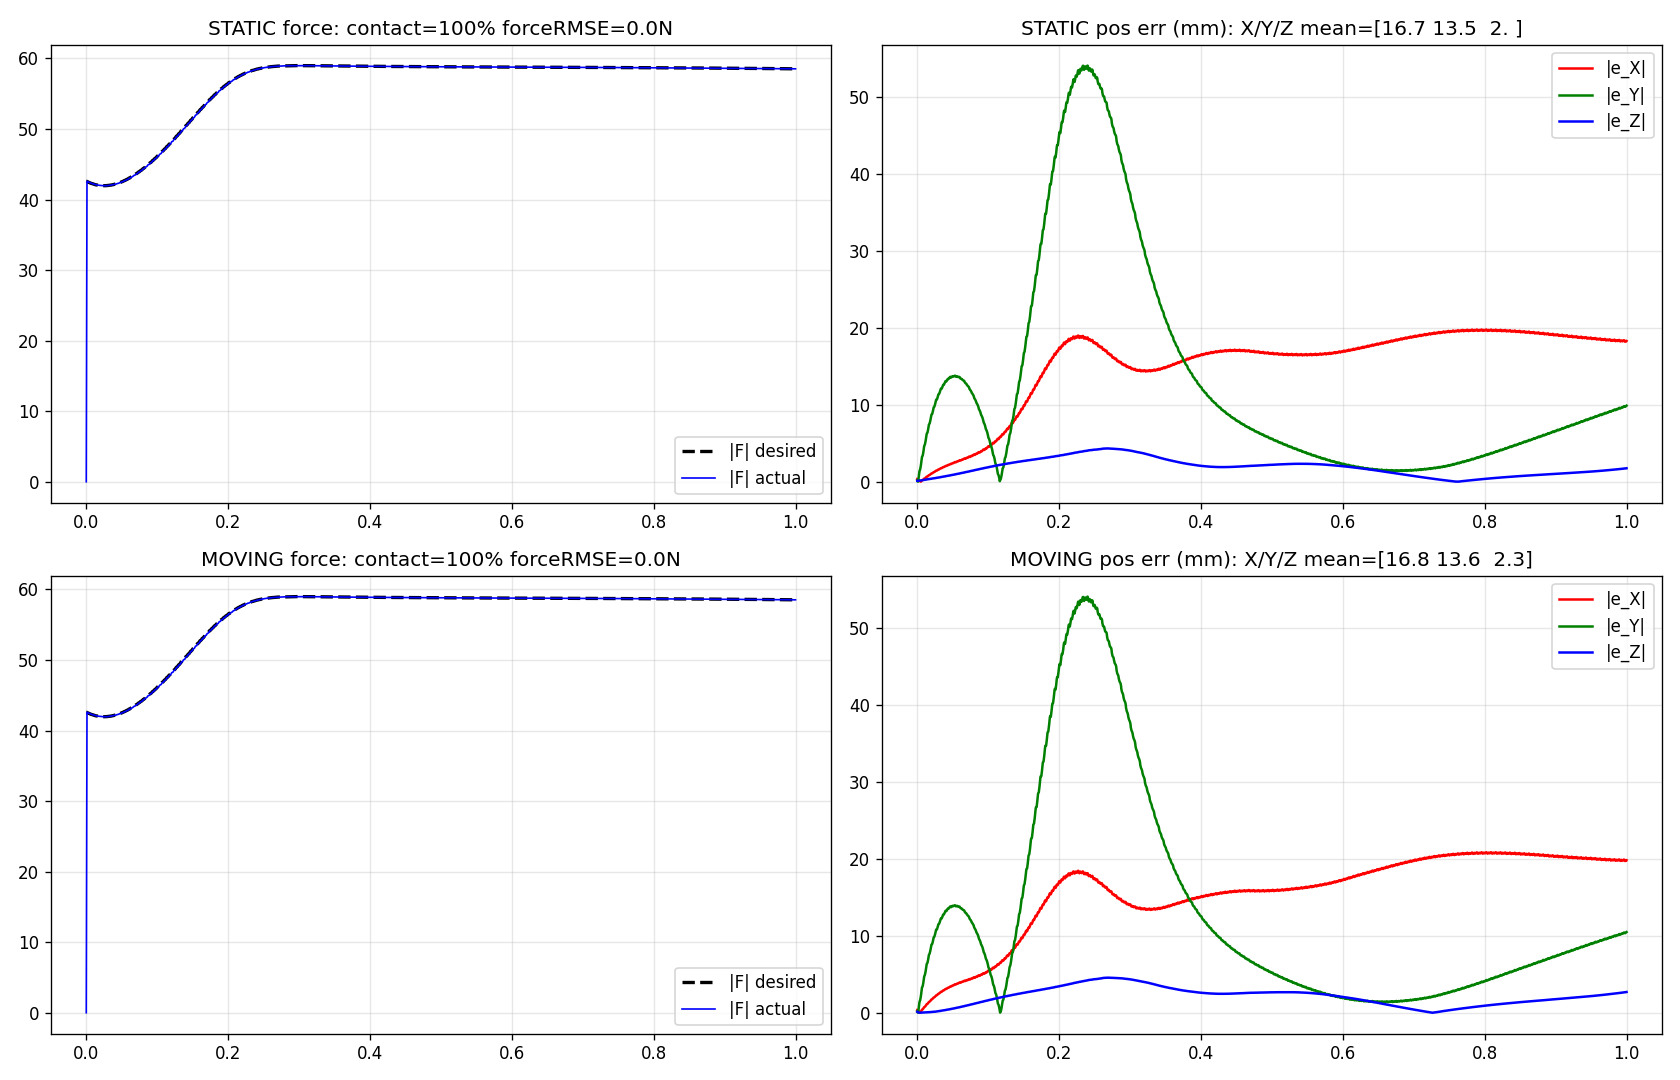
\includegraphics[width=0.97\textwidth]{cut_calibrated.png}
\caption{Cutting with the identified material model on \textbf{cork}. Left column:
the measured contact-force magnitude (blue) follows the desired (dashed) for the
whole cut, on static (top) and moving (bottom) workpieces. Right column: per-axis
position error --- the cut-depth (Z) error stays $\approx2$\,mm; the lateral (Y)
error peaks during the large demonstrated lateral swing.}
\label{fig:calibrated}
\end{figure}

Figure~\ref{fig:calibrated_others} reports the earlier material-model replay for
PVC and penoplex. Those plots assess consistency of a model identified from the
same demonstrations; they are not independent evidence of force-regulation
accuracy. Moreover, their moving-workpiece traces were generated under an
earlier reference convention and are not used to support the fixed-world
reference ablation of Section~\ref{sec:holdback}.

\begin{figure}[h]
\centering
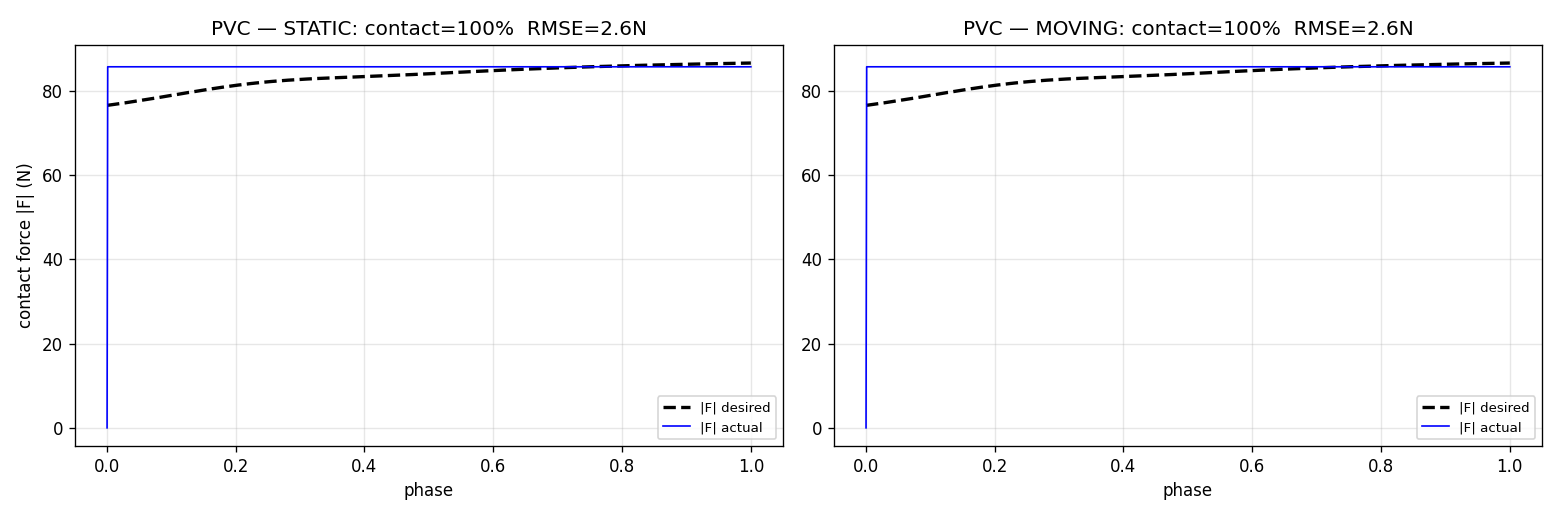
\includegraphics[width=0.93\textwidth]{cut_calibrated_pvc.png}\\[4pt]
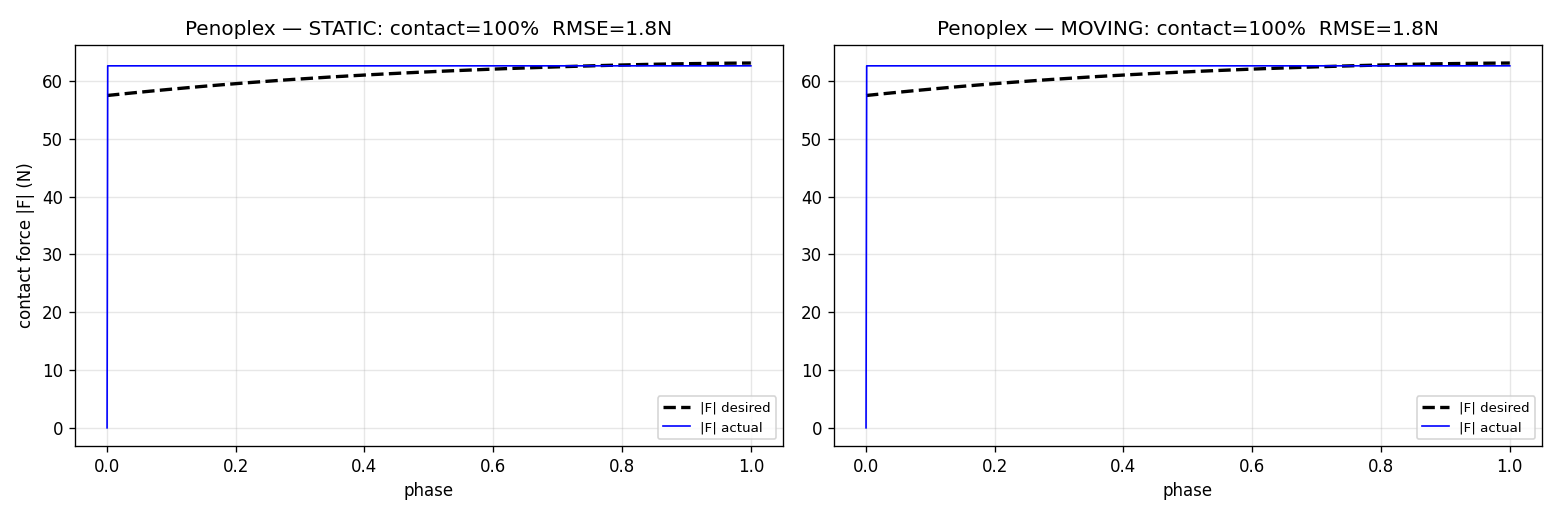
\includegraphics[width=0.93\textwidth]{cut_calibrated_peno.png}
\caption{Force tracking on \textbf{PVC} (top) and \textbf{penoplex} (bottom),
static (left) and moving (right). The measured force (blue) follows each
material's demonstrated level (dashed) to $\approx2$\,N RMSE with $100\%$ contact.
PVC plateaus highest ($\sim86$\,N, hardest material), penoplex lowest
($\sim63$\,N), mirroring the per-material cutting parameters of
Table~\ref{tab:material}.}
\label{fig:calibrated_others}
\end{figure}

\begin{itemize}[leftmargin=1.5em]
\item \textbf{The task performance is attributable to the learned variance
structure} (Table~\ref{tab:variance_comparison},
Fig.~\ref{fig:variance_comparison}): the identified
precision attains the lowest cut-depth error --- $26$--$48\%$ below the inverted,
permuted, and direct-force assignments --- on every stable seed ($p=0.001$).
\item \textbf{Material-model replay} (Table~\ref{tab:material},
Fig.~\ref{fig:calibrated}): the identified reaction reproduces the demonstrated
force scale in the calibration setting. Because identification and assessment
use the same demonstration source, this is a consistency check rather than an
independent force-control validation.
\item \textbf{Position tracking}: deterministic nominal cut-depth RMSE is
$1.776$--$2.384$\,mm in the four-case cork comparison. Full Cartesian error is
larger, and the 120\,N holdback produces $51.952$--$83.208$\,mm RMSE; no
high-precision Cartesian tracking claim is made.
\item \textbf{Passivity} (Fig.~\ref{fig:pass_adv}, Table~\ref{tab:pass_adv}):
under positive joint-power perturbation, the controller without tank projection
violates the available energy budget for $65.4\%$ of the samples
($+20{,}239$\,W maximum margin), while both tanked controllers satisfy
$\dot q^\top\tau_{\rm safe}\le P_{\max}$ for the whole run. With the deliberately
small 1\,J stress-test tank, the phase-gated case halts at $\phi=0.250$ rather
than completing.
\item \textbf{Stability diagnostics} (Fig.~\ref{fig:stab}): nominal static and
moving cuts remain bounded and complete the task; cut-depth error stays small.
The exponential fit is reported as a diagnostic, while the full Cartesian error
norm is interpreted carefully because low-precision axes are intentionally
released.
\item \textbf{Run monitoring}: Figure~\ref{fig:monitor} shows the monitored
signals for static and moving workpieces, with the validation holdback disabled
and enabled: position, material reaction, stiffness, tracking error and tank
energy, each in its own units.
\end{itemize}

\begin{figure}[h]
\centering
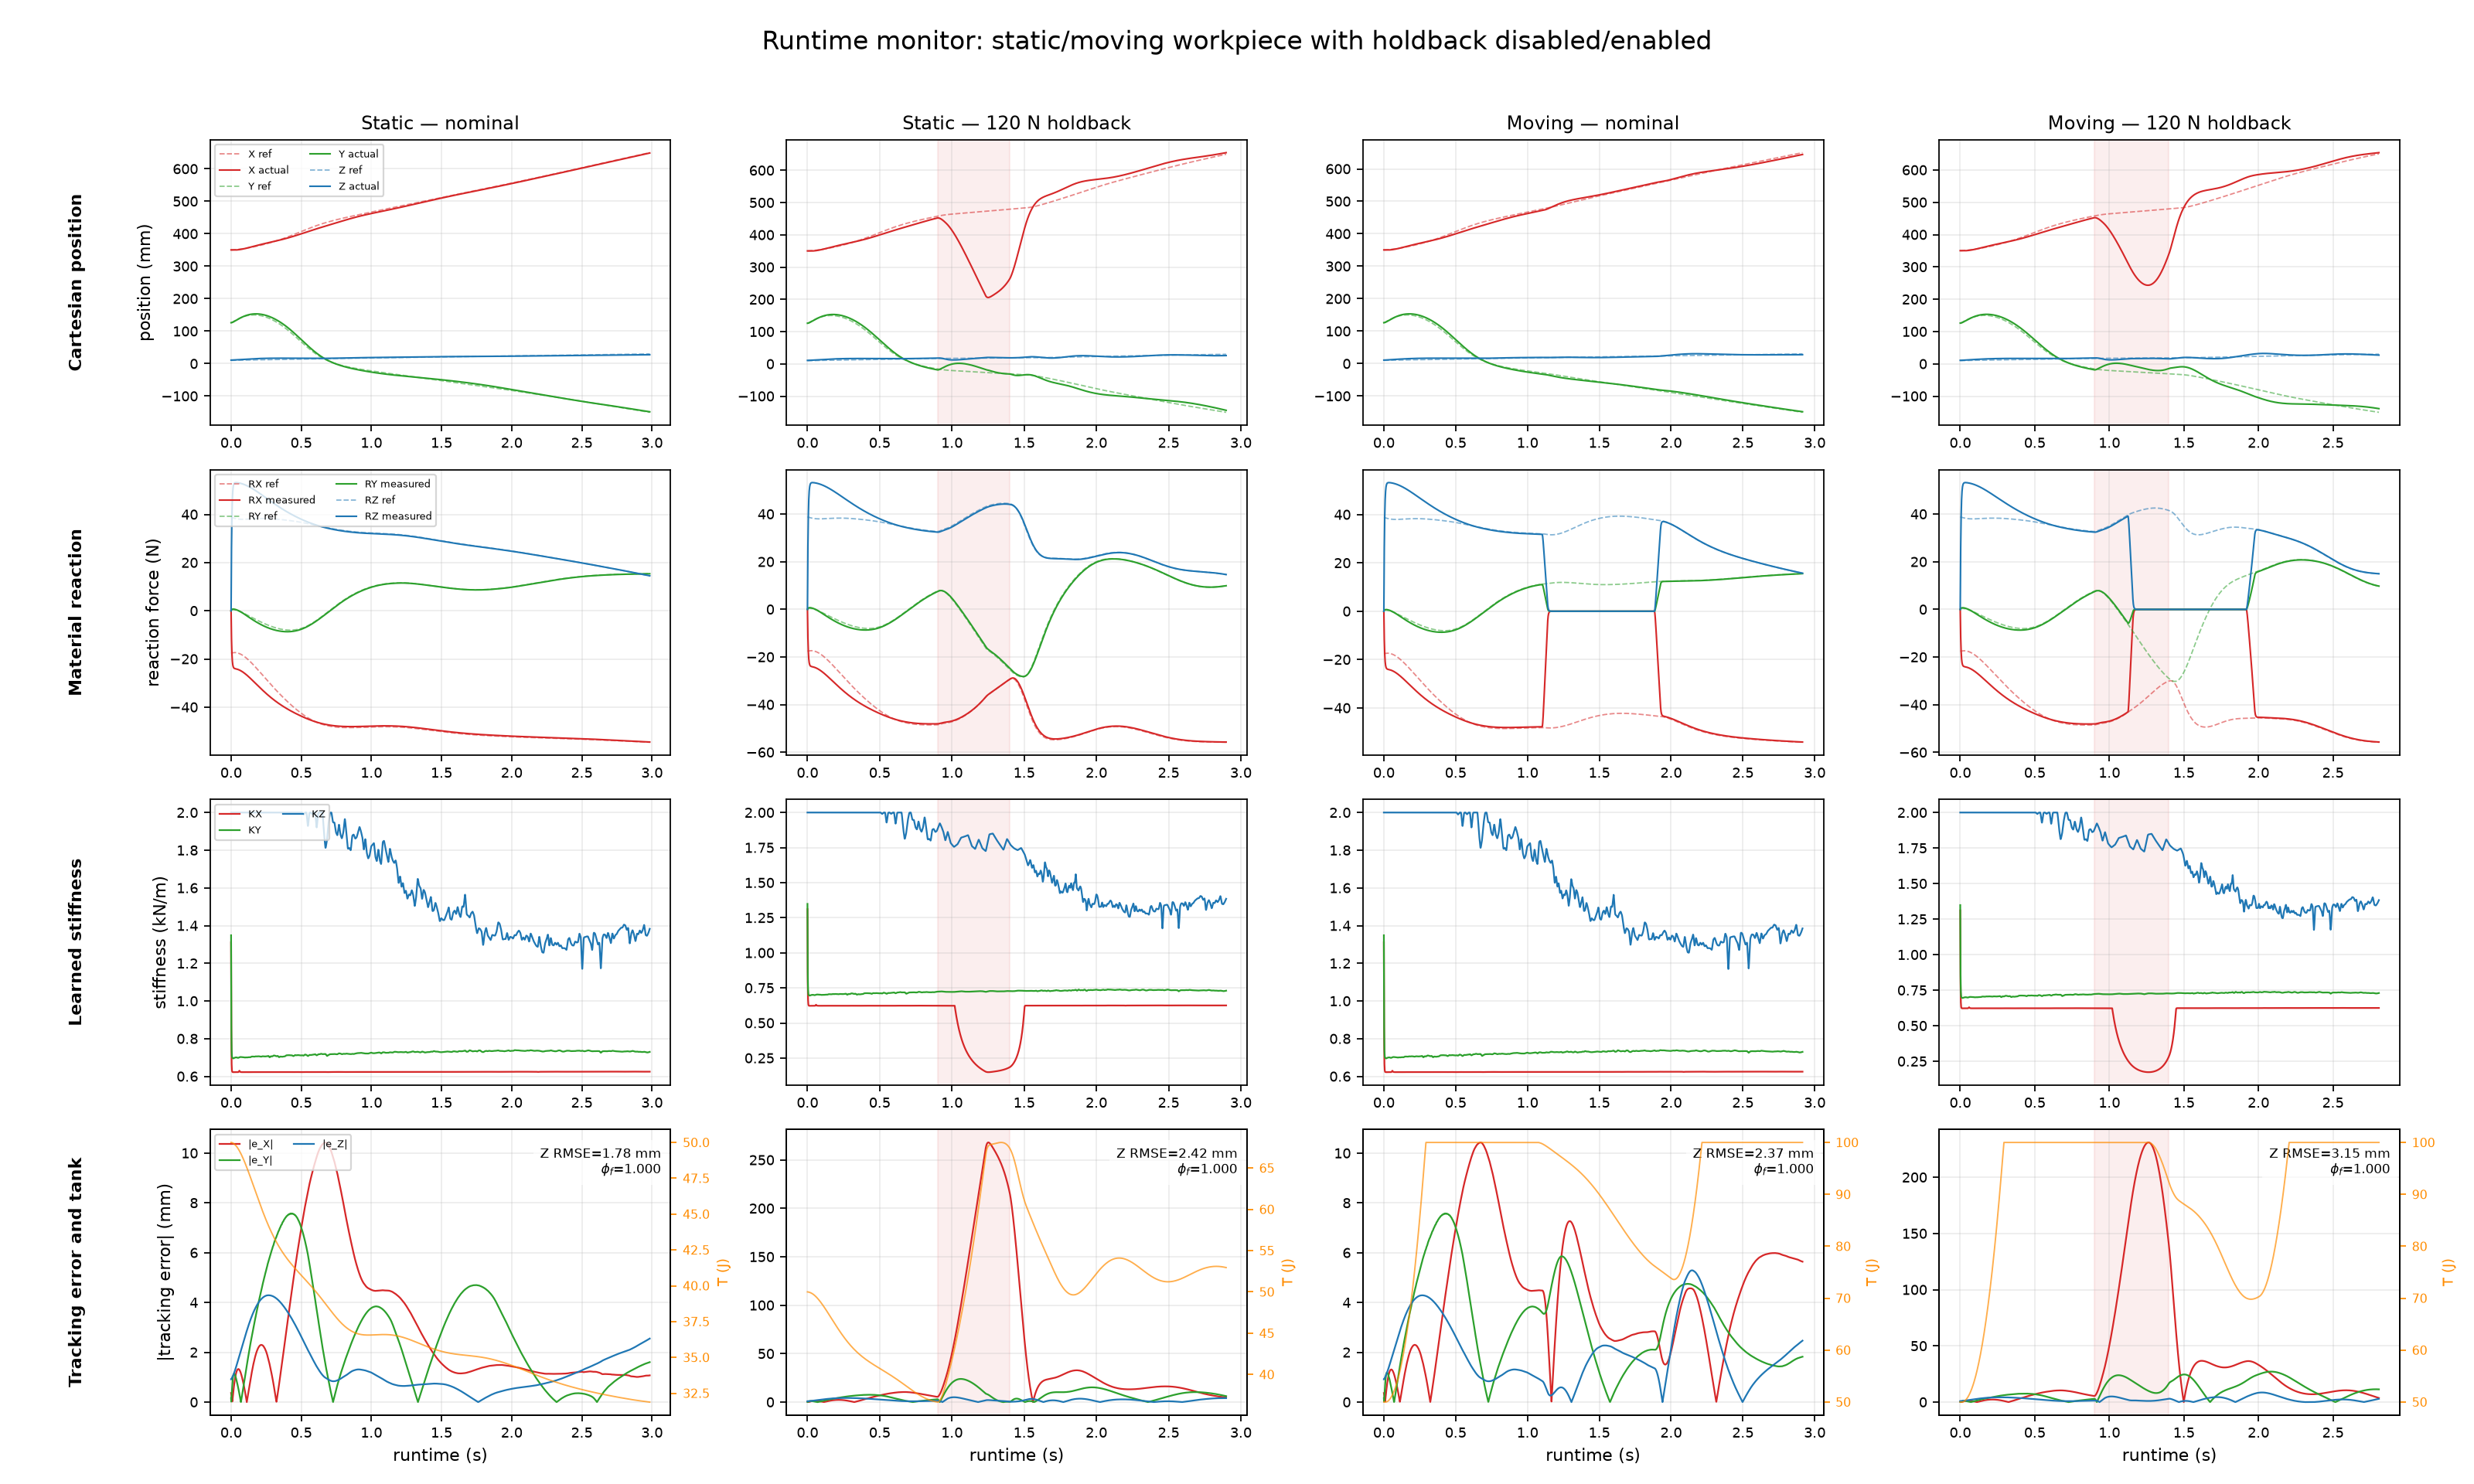
\includegraphics[width=\textwidth]{monitor_preview.png}
\caption{Runtime monitor reconstructed from four state-driven cork episodes:
static nominal, static with $120$\,N holdback, moving nominal, and moving with
holdback (columns from left to right). Rows show Cartesian position,
axis-resolved material reaction, learned stiffness, and absolute tracking error
with tank energy. Red shading identifies the validation-force interval
$[0.9,1.4]$\,s; the plotted reaction channel remains the identified material
reaction and does not re-label the separately applied holdback as contact
force. The desired world-frame path is common to all columns, although its
time-indexed samples differ when state-driven phase timing changes.
Representative cut-depth RMSE is $1.776$, $2.424$, $2.372$ and $3.148$\,mm,
respectively. The holdback columns exhibit large Cartesian displacement and
must be interpreted as stress tests rather than precision-tracking results.}
\label{fig:monitor}
\end{figure}

% ============================================================================
\section{Novelty and contributions}
% ============================================================================
\begin{enumerate}[leftmargin=1.7em]
\item \textbf{Gains learned from demonstration precision, via an online QP.}
Stiffness \emph{is} the demonstration precision \eqref{eq:precision}, computed each
step by the QP \eqref{eq:qp} that blends force-consistency with precision-stiffness
under force-saturation constraints. The controlled comparison
(Table~\ref{tab:variance_comparison}) shows
the \emph{specific} learned variance structure --- not generic adaptivity --- is
what carries the skill.
\item \textbf{State-driven task parametrisation.} A phase variable advanced by
matching the robot's measured state to the prior \eqref{eq:phase}, rather than by a
clock, giving speed-adaptability and disturbance awareness, and unifying with the
stability mechanism.
\item \textbf{Torque-port passivity under variable gains and a moving target.}
The live energy tank sets the torque-level power budget \eqref{eq:pass_qp};
Fig.~\ref{fig:pass_adv} demonstrates that this rejects positive-power
perturbations. A cross-term Lyapunov proof (Theorem~\ref{thm:exp}) gives the
exponential-contraction condition for the regulated error dynamics, and the tank
provides the mechanism that bounds phase and gain rates.
\item \textbf{An empirical principle for contact-skill transfer.} Position is the
reproducible prior, force is not; the controller therefore regulates position and
treats force as a constraint, while a per-material identified model supplies the
interaction force.
\end{enumerate}

% ============================================================================
\section{Assumptions, scope and limitations}
% ============================================================================
\begin{itemize}[leftmargin=1.5em]
\item The contact \emph{force} matches because the material model is identified to
the demonstration (system identification); the \emph{controller} achieves the
position/velocity tracking. These two roles are reported separately, and the force
result is \emph{not} presented as controller force-tracking.
\item All experiments are in simulation; the material parameters are identified
from the real material's measured demonstration forces. Real-robot validation is
future work.
\item Lateral (Y) tracking lags the large demonstrated lateral swing; the
task-critical cut-depth is tight. Reducing the lateral error is a
phase-speed / parametrisation question, separate from the force model.
\item The energy-tank passivity guarantee is implemented and validated at the
joint torque port. The reconstructed Cartesian residual is retained as a useful
diagnostic, but it is not the primary proof artifact until the force frame/sign,
finite-difference velocity estimate and Cartesian storage model are matched more
precisely.
\item The exponential-stability proof applies under regulation assumptions
(constant or sufficiently slowly varying gains, passive environment, bounded
reference acceleration). The current simulations support bounded stable cutting;
a stronger empirical exponential-convergence claim should be made on the
regulated cut-depth or precision-weighted error, not on the full Cartesian norm
that includes intentionally released axes.
\end{itemize}

\end{document}
